\documentclass[12pt, oneside]{article}

\usepackage[letterpaper, scale=0.89, centering]{geometry}
\usepackage{fancyhdr}
\setlength{\parindent}{0em}
\setlength{\parskip}{1em}

\pagestyle{fancy}
\fancyhf{}
\renewcommand{\headrulewidth}{0pt}
\rfoot{\href{https://creativecommons.org/licenses/by-nc-sa/2.0/}{CC BY-NC-SA 2.0} Version \today~(\thepage)}

\usepackage{amssymb,amsmath,pifont,amsfonts,comment,enumerate,enumitem}
\usepackage{currfile,xstring,hyperref,tabularx,graphicx,wasysym}
\usepackage[labelformat=empty]{caption}
\usepackage[dvipsnames,table]{xcolor}
\usepackage{multicol,multirow,array,listings,tabularx,lastpage,textcomp,booktabs}

\lstnewenvironment{algorithm}[1][] {   
    \lstset{ mathescape=true,
        frame=tB,
        numbers=left, 
        numberstyle=\tiny,
        basicstyle=\rmfamily\scriptsize, 
        keywordstyle=\color{black}\bfseries,
        keywords={,procedure, div, for, to, input, output, return, datatype, function, in, if, else, foreach, while, begin, end, }
        numbers=left,
        xleftmargin=.04\textwidth,
        #1
    }
}
{}
\lstnewenvironment{java}[1][]
{   
    \lstset{
        language=java,
        mathescape=true,
        frame=tB,
        numbers=left, 
        numberstyle=\tiny,
        basicstyle=\ttfamily\scriptsize, 
        keywordstyle=\color{black}\bfseries,
        keywords={, int, double, for, return, if, else, while, }
        numbers=left,
        xleftmargin=.04\textwidth,
        #1
    }
}
{}

\newcommand\abs[1]{\lvert~#1~\rvert}
\newcommand{\st}{\mid}

\newcommand{\A}[0]{\texttt{A}}
\newcommand{\C}[0]{\texttt{C}}
\newcommand{\G}[0]{\texttt{G}}
\newcommand{\U}[0]{\texttt{U}}

\newcommand{\cmark}{\ding{51}}
\newcommand{\xmark}{\ding{55}}

 
\begin{document}
\begin{flushright}
    \StrBefore{\currfilename}{.}
\end{flushright} \section*{Netflix intro}


What data should we encode about each Netflix account holder to help us make effective recommendations?

\vfill
\vfill

In machine learning, clustering can be used to group similar data for prediction and recommendation.  For example,
each Netflix user's viewing history can be represented as a $n$-tuple indicating their preferences about
movies in the database, where $n$ is the number of movies in the database.  People with similar tastes in movies can then be clustered to provide recommendations
of movies for one another.  Mathematically, clustering is based on a notion of distance between pairs of $n$-tuples.
 \vfill
\section*{Data types}


\begin{center}
    \begin{tabular}{p{4.6in}p{2.6in}}
    {\bf  Term} & {\bf Examples}:\\
    &  (add additional examples from class)\\
    \hline 
    {\bf set} \newline
    unordered collection of elements & $7 \in \{43, 7, 9 \}$ \qquad $2 \notin \{43, 7, 9 \}$ \\
    {\it repetition doesn't matter} & \\
    {\it Equal sets agree on membership of all elements}& \\
    \hline
    {\bf $n$-tuple} \newline
    ordered sequence of elements with $n$ ``slots" ($n >0$) & \\
    {\it repetition matters, fixed length} &\\
    {\it Equal $n$-tuples have corresponding components equal}& \\
    \hline
    {\bf string} \newline
    ordered finite sequence of elements each from specified
    set & \\
    {\it repetition matters, arbitrary finite length} &\\
    {\it Equal strings have same length and corresponding characters equal}
    \end{tabular}
\end{center}

{\it Special cases}: 

When $n=2$, the 2-tuple is called an {\bf ordered pair}.

A string of length $0$ is called the {\bf empty string} and is denoted $\lambda$.

A set with no elements is called the {\bf empty set} and is denoted $\{\}$ or $\emptyset$. \vfill
\section*{Set operations}


\fbox{\parbox{\textwidth}{To define a set we can use the roster method, set builder notation, a recursive definition, 
and also we can apply a set operation to other sets. \\

{\bf New! Cartesian product of sets} and {\bf set-wise concatenation of sets of strings}\\


{\bf Definition}: Let $X$ and $Y$ be sets.  The {\bf Cartesian product} of $X$ and $Y$, denoted
$X \times Y$, is the set of all ordered pairs $(x,y)$ where $x \in X$ and $y \in Y$
\[
X \times Y = \{ (x,y) \mid x \in X \text{ and } y \in Y \}
\]
{\bf Definition}: Let $X$ and $Y$ be sets of strings over the same alphabet. The {\bf set-wise concatenation} 
of $X$ and $Y$, denoted $X \circ Y$, is the set of all results of string concatenation $xy$ where $x \in X$ 
and $y \in Y$
\[
X \circ Y = \{ xy \mid x \in X \text{ and } y \in Y \}
\]
}}

{\bf Pro-tip}: the meaning of writing one element next to another like $xy$ depends on the data-types of $x$ and 
$y$. When $x$ and $y$ are strings, the convention is that $xy$ is the result of string concatenation. 
When $x$ and $y$ are numbers, the convention is that $xy$ is the result of multiplication. This is 
(one of the many reasons) why is it very important to declare the data-type of variables before we use them.

{\it Fill in the missing entries in the table}:

\begin{center}
\begin{tabular}{cc}
{\bf  Set} & {\bf Example elements in this set}:\\
\hline 
& \\
$B$ &\A \qquad \C \qquad \G \qquad \U \\
& \\
\hline
& \\
\phantom{$B \times B$} & $(\A, \C)$ \qquad $(\U, \U)$\\
& \\
\hline
& \\
$B \times \{-1,0,1\}$ & \\
& \\
\hline
& \\
$\{-1,0,1\} \times B$ & \\
& \\
\hline
& \\
\phantom{$\{-1,0,1\} \times \{-1,0,1\}  \times \{-1,0,1\} $} & \qquad $(0,0,0)$ \\
& \\
\hline
& \\
$ \{\A, \C, \G, \U \} \circ  \{\A, \C, \G, \U \}$& \\
& \\
\hline
& \\
\phantom{$\{G\} \circ \{G\} \circ \{G\}$} & \qquad $\G\G\G\G$ \\
& \\
\hline

\end{tabular}
\end{center}

\vfill \vfill
\section*{Defining functions}


\fbox{\parbox{\textwidth}{{\bf New! Defining functions} A function is defined by its (1) domain, 
(2) codomain, and (3) rule assigning each 
element in the domain exactly one element in the codomain.\\

The domain and codomain are nonempty sets.

The rule can be depicted as a table, formula, or English description.

The notation is 
\begin{center}
    ``Let the function FUNCTION-NAME: DOMAIN $\to$ CODOMAIN be given by \\
FUNCTION-NAME(x) = \ldots for every $x \in DOMAIN$''.
\end{center}

or 
\begin{center}
    ``Consider the function FUNCTION-NAME: DOMAIN $\to$ CODOMAIN given by \\
FUNCTION-NAME(x) = \ldots for every $x \in DOMAIN$''.
\end{center}
}}

\vfill

Example: The absolute value function 

{\bf Domain}

{\bf Codomain}

{\bf Rule}

\vfill 
 \vfill
\section*{Defining functions recursively}


When the domain of a function is a {\it recursively defined set}, the rule assigning 
images to domain elements (outputs) can also be defined recursively.

Recall: The set of RNA strands $S$ is defined (recursively) by:
\[
\begin{array}{ll}
\textrm{Basis Step: } & \A \in S, \C \in S, \U \in S, \G \in S \\
\textrm{Recursive Step: } & \textrm{If } s \in S\textrm{ and }b \in B \textrm{, then }sb \in S
\end{array}
\]
where $sb$ is string concatenation.

{\bf Definition} (Of a function, recursively) A function \textit{rnalen} that computes the length of RNA strands in $S$ is defined by:
\[
\begin{array}{llll}
& & \textit{rnalen} : S & \to \mathbb{Z}^+ \\
\textrm{Basis Step:} & \textrm{If } b \in B\textrm{ then } & \textit{rnalen}(b) & = 1 \\
\textrm{Recursive Step:} & \textrm{If } s \in S\textrm{ and }b \in B\textrm{, then  } & \textit{rnalen}(sb) & = 1 + \textit{rnalen}(s)
\end{array}
\]

The domain of \textit{rnalen} is \phantom{$S$}\\

The codomain of \textit{rnalen} is \phantom{$\mathbb{Z}^+$}\\

Example function application:
\[
rnalen(\A\C\U) = \phantom{1+ rnalen(\A\C) = 1 + (1 + rnalen(\A) ) = 1 + ( 1 + 1) = 3}
\]

\vfill

{\it Extra example}: A function \textit{basecount} that computes the number of a given base 
$b$ appearing in a RNA strand $s$ is defined recursively:
    
\[
\begin{array}{llll}
& & \textit{basecount} : S \times B & \to \mathbb{N} \\
\textrm{Basis Step:} &  \textrm{If } b_1 \in B, b_2 \in B & \textit{basecount}(~(b_1, b_2)~) & =
        \begin{cases}
            1 & \textrm{when } b_1 = b_2 \\
            0 & \textrm{when } b_1 \neq b_2 \\
        \end{cases} \\
\textrm{Recursive Step:} & \textrm{If } s \in S, b_1 \in B, b_2 \in B &\textit{basecount}(~(s b_1, b_2)~) & =
        \begin{cases}
            1 + \textit{basecount}(~(s, b_2)~) & \textrm{when } b_1 = b_2 \\
            \textit{basecount}(~(s, b_2)~) & \textrm{when } b_1 \neq b_2 \\
        \end{cases}
\end{array}
\]

$basecount(~(\A\C\U,\A)~) = basecount( ~(\A\C, \A)~) = basecount(~(\A, \A)~) = 1$\\


$basecount(~(\A\C\U,\G)~) = basecount( ~(\A\C, \G)~) = basecount(~(\A, \G)~) = 0$\\


\vfill
{\it Extra example}: The function which outputs $2^n$ when given a nonnegative integer $n$ can be defined recursively, 
because its domain is the set of nonnegative integers.

\vfill
 \vfill
\section*{Why represent numbers}


Modeling uses data-types that are 
encoded in a computer.

The details of the encoding impact the efficiency of algorithms
we use to understand the systems we are modeling and the 
impacts of these algorithms on the people using the systems.

Case study: how to encode numbers?

\phantom{
Positional representation with familiar (decimal) number encodings
\vspace{30pt}
}
\vfill \vfill
\section*{Base expansion definition}


{\bf Definition} For $b$ an integer greater than $1$ and $n$ a positive integer, 
the {\bf base $b$ expansion of $n$}  is
\[
(a_{k-1} \cdots a_1 a_0)_b
\]
where $k$ is a positive integer, $a_0, a_1, \ldots, a_{k-1}$ 
are nonnegative integers less than $b$, $a_{k-1} \neq  0$, and
\[
n =  \sum_{i=0}^{k-1} a_{i} b^{i}
\]

Notice: {\it The base $b$ expansion of a positive integer $n$ is a string over the alphabet 
$\{x \in \mathbb{N} \st x < b\}$
whose leftmost character is nonzero.}

\begin{center}
\begin{tabular}{|c|c|}
\hline
Base $b$ & Collection of possible coefficients in base $b$ expansion of  a positive integer \\
\hline
& \\
Binary ($b=2$) & $\{0,1\}$ \\
\hline
& \\
Ternary ($b=3$) & $\{0,1, 2\}$ \\
\hline
& \\
Octal ($b=8$) & $\{0,1, 2, 3, 4, 5, 6, 7\}$\\
\hline
& \\
Decimal ($b=10$) & $\{0,1, 2, 3, 4, 5, 6, 7, 8, 9\}$\\
\hline
& \\
Hexadecimal ($b=16$) &  $\{0,1, 2, 3, 4, 5, 6, 7, 8, 9, A, B, C, D, E, F\}$\\
& letter coefficient symbols represent numerical values $(A)_{16} = (10)_{10}$\\
&$(B)_{16} = (11)_{10} ~~(C)_{16} = (12)_{10} ~~
 (D)_{16} = (13)_{10} ~~ (E)_{16} = (14)_{10} ~~ (F)_{16} = (15)_{10} $\\
\hline
\end{tabular}
\end{center}

 \vfill
\section*{Base expansion examples}


\fbox{\parbox{\textwidth}{{\bf Common bases}: \hfill Binary  $b=2$ \qquad Octal $b=8$ \qquad Decimal $b=10$ \qquad Hexadecimal $b=16$
\hfill }}

{\it Examples}:

$(1401)_{2}$

\vfill

$(1401)_{10}$

\vfill
\vfill
\vfill


$(1401)_{16}$

\vfill
\vfill
\vfill
 \vfill
\section*{Algorithm definition}


\fbox{\parbox{\textwidth}{{\bf New!} An algorithm is a finite sequence of precise instructions for solving a problem.
\hfill
}} \vfill
\section*{Algorithm half}


\begin{algorithm}[caption={Algorithm for calculating integer part of half the input}]
    procedure $\textit{half}$($n$: a positive integer)
    $r$ := $0$
    while $n$ > $1$
      $r$ := $r + 1$
      $n$ := $n - 2$
    return $r$ $\{ r~\textrm{holds the result of the operation}\} $
    \end{algorithm}

 \begin{multicols}{2}
  \begin{center} 
    \begin{tabular}{c|c|c}
    $n$ & $r$  & $n > 1$?\\
    \hline 
    ~$6$~ & \phantom{~$0$~} & \phantom{~T~}\\
    \phantom{$4$} & \phantom{$1$} & \phantom{T}\\
    \phantom{$2$} & \phantom{$2$} & \phantom{T}\\
    \phantom{$0$} & \phantom{$3$} & \phantom{F}\\
    &\\
    \end{tabular}
    \end{center}
    \begin{center}
      \begin{tabular}{c|c|c}
      $n$ & $r$  & $n > 1$?\\
      \hline 
      ~$5$~ & \phantom{~$0$~} & \phantom{~T~}\\
      \phantom{$3$} & \phantom{$1$} & \phantom{T}\\
      \phantom{$1$} & \phantom{$2$} & \phantom{F}\\
      &\\
      \end{tabular}
      \end{center}    
\end{multicols}

\vfill \vfill
\section*{Algorithm log}


 \begin{algorithm}[caption={Algorithm for calculating integer part of $\log$}]
    procedure $\textit{log}$($n$: a positive integer)
    $r$ := $0$
    while $n$ > $1$
      $r$ := $r + 1$
      $n$ := $half(n)$
    return $r$ $\{ r~\textrm{holds the result of the}~\log~\textrm{operation}\} $
\end{algorithm}

\begin{multicols}{2}
  \begin{center}
    \begin{tabular}{c|c|c}
    $n$ & $r$  & $n > 1$?\\
    \hline 
    ~$8$~ & \phantom{~$0$~} & \phantom{~T~}\\
    \phantom{$4$} & \phantom{$1$} & \phantom{T}\\
    \phantom{$2$} & \phantom{$2$} & \phantom{T}\\
    \phantom{$1$} & \phantom{$3$} & \phantom{F}\\
    &\\
    \end{tabular}
    \end{center}
  \begin{center}
    \begin{tabular}{c|c|c}
    $n$ & $r$  & $n > 1$?\\
    \hline 
    ~$6$~ & \phantom{~$0$~} & \phantom{~T~}\\
    \phantom{$3$} & \phantom{$1$} & \phantom{T}\\
    \phantom{$1$} & \phantom{$2$} & \phantom{F}\\
    &\\
    \end{tabular}
    \end{center}
\end{multicols}

\vfill

\fbox{\parbox{\textwidth}{
$2^0 = 1$~~\hfill $2^1=2$~~\hfill $2^2=4$~~\hfill $2^3=8$~~
\hfill $2^4=16$~~\hfill $2^5=32$~~
\hfill $2^6=64$~~\hfill $2^7=128$~~
\hfill $2^8=256$~~\hfill $2^9=512$~~
\hfill $2^{10}=1024$}} \vfill
\section*{Division algorithm}


{\bf Integer division and remainders} (aka The Division Algorithm) Let $n$ be an integer 
and $d$ a positive integer. There are unique integers $q$ and $r$, with $0 \leq r < d$, such that 
$n = dq + r$. In this case, $d$ is called the divisor, $n$ is called the dividend, 
$q$ is called the quotient, 
and $r$ is called the remainder. We write $q=n \textbf{ div } d$ and $r=n \textbf{ mod } d$.

\textit{Extra example}: How do $\textbf{ div }$ and $\textbf{ mod }$ compare to $/$ and $\%$ in Java and python?

\vfill
 \vfill
\section*{Base expansion algorithms}


{\bf Two algorithms for constructing base $b$ expansion from decimal representation}

{\bf Most significant first}: Start with left-most coefficient of expansion
\begin{multicols}{2}
\begin{algorithm}[caption={Calculating integer part of $\log_b$}]
procedure $\textit{logb}$($n, b$: positive integers with $b > 1$)
$r$ := $0$
while $n$ > $b-1$
  $r$ := $r + 1$
  $n$ := $n$ div $b$
return $r$ $\{ r~\textrm{holds the result of the}~\log_b~\textrm{operation}\}$
\end{algorithm}
\columnbreak
\begin{algorithm}[caption={Calculating base $b$ expansion, from left}]
procedure $\textit{baseb1}$($n, b$: positive integers with $b > 1$)
$v$ := $n$
$k$ := $logb(n,b) + 1$
for $i$ := $1$ to $k$
  $a_{k-i}$ := $0$
  while $v \geq b^{k-i}$
    $a_{k-i}$ := $a_{k-i} + 1$
    $v$ := $v -  b^{k-i}$
return $(a_{k-1}, \ldots, a_0) \{(a_{k-1} \ldots a_0)_b~\textrm{ is the base } b \textrm{ expansion of } n \}$
\end{algorithm}
\end{multicols}

\vfill
\vfill

{\bf Least significant first}: Start with right-most coefficient of expansion

\begin{multicols}{2}
  \begin{minipage}{3.2in}
    Idea: {\tiny(when $k > 1$)} 
    \begin{align*}
      n &= a_{k-1} b^{k-1} + \cdots + a_1 b + a_0 \\
        &= b ( a_{k-1} b^{k-2} + \cdots + a_1) + a_0\end{align*}
    so $a_0 = n \textbf{ mod } b$ and $a_{k-1} b^{k-2} + \cdots + a_1 = n \textbf{ div } b$.

\end{minipage}
\columnbreak
\begin{algorithm}[caption={Calculating base $b$ expansion, from right}]
procedure $\textit{baseb2}$($n, b$: positive integers with $b > 1$)
$q$ := $n$
$k$ := $0$
while $q  \neq 0$
  $a_{k}$ := $q$ mod $b$
  $q$ := $q$ div $b$
  $k$ := $k+1$
return $(a_{k-1}, \ldots, a_0) \{(a_{k-1} \ldots a_0)_b~\textrm{ is the base } b \textrm{ expansion of } n \}$
\end{algorithm}
\end{multicols}

\vfill
\vfill \vfill
\section*{Base expansion review}


Find and fix any and all mistakes with the following:
\begin{itemize}
\item[(a)] $(1)_2 = (1)_8$
\item[(b)] $(142)_{10} = (142)_{16}$
\item[(c)] $(20)_{10} = (10100)_2$
\item[(d)] $(35)_8 = (1D)_{16}$
\end{itemize} \vfill
\section*{Base conversion algorithm}


{\it Recall the definition of base expansion we discussed:}



{\bf Definition} For $b$ an integer greater than $1$ and $n$ a positive integer, 
the {\bf base $b$ expansion of $n$}  is
\[
(a_{k-1} \cdots a_1 a_0)_b
\]
where $k$ is a positive integer, $a_0, a_1, \ldots, a_{k-1}$ 
are nonnegative integers less than $b$, $a_{k-1} \neq  0$, and
\[
n =  \sum_{i=0}^{k-1} a_{i} b^{i}
\]

Notice: {\it The base $b$ expansion of a positive integer $n$ is a string over the alphabet 
$\{x \in \mathbb{N} \st x < b\}$
whose leftmost character is nonzero.}

\begin{center}
\begin{tabular}{|c|c|}
\hline
Base $b$ & Collection of possible coefficients in base $b$ expansion of  a positive integer \\
\hline
& \\
Binary ($b=2$) & $\{0,1\}$ \\
\hline
& \\
Ternary ($b=3$) & $\{0,1, 2\}$ \\
\hline
& \\
Octal ($b=8$) & $\{0,1, 2, 3, 4, 5, 6, 7\}$\\
\hline
& \\
Decimal ($b=10$) & $\{0,1, 2, 3, 4, 5, 6, 7, 8, 9\}$\\
\hline
& \\
Hexadecimal ($b=16$) &  $\{0,1, 2, 3, 4, 5, 6, 7, 8, 9, A, B, C, D, E, F\}$\\
& letter coefficient symbols represent numerical values $(A)_{16} = (10)_{10}$\\
&$(B)_{16} = (11)_{10} ~~(C)_{16} = (12)_{10} ~~
 (D)_{16} = (13)_{10} ~~ (E)_{16} = (14)_{10} ~~ (F)_{16} = (15)_{10} $\\
\hline
\end{tabular}
\end{center}

 
We write an algorithm for converting from base $b_1$ expansion to base $b_2$ expansion:

\phantom{
Earlier, we saw (two different) algorithms for, given 
a target base $b$, converting from decimal to base $b$ expansions. 
We will use either one of these as a subroutine in this algorithm.\\
Given a base expansion in base $b_1$:\\
Step 1: Use the definition of base expansion to calculate the value of
    this number (in decimal).\\
Step 2: Use the Least Significant First algorithm to write this value in 
    base $b_2$ and output the result.
}
\vspace{200pt} \vfill
\section*{Fixed width definition}


{\bf Definition} For $b$ an integer greater than $1$, $w$ a positive integer, 
and $n$ a nonnegative integer
$\underline{\phantom{\hspace{1in}}}$, ~
the {\bf base $b$ fixed-width $w$ expansion of $n$}  is
\[
(a_{w-1} \cdots a_1 a_0)_{b,w}
\]
where  $a_0, a_1, \ldots, a_{w-1}$ are nonnegative integers less than $b$ and
\[
n =  \sum_{i=0}^{w-1} a_{i} b^{i}
\]
 \vfill
\section*{Fixed width example}


\begin{center}
    \begin{tabular}{|c|c|c|c|c|}
    \hline
    Decimal &  Binary  & Binary fixed-width $10$& Binary fixed-width $7$ & Binary fixed-width $4$\\
    $b=10$ & $b=2$ & $b=2$, $w =  10$& $b=2$, $w =  7$& $b=2$, $w =  4$ \\
    \hline 
    &&&&  \\
    $(20)_{10}$&\phantom{$(10100)_{2}$\qquad\qquad}&&  &\\
    &&&&  \\
    &(a)&(b)&(c)&(d)  \\
    \hline
    \end{tabular}
    \end{center}
 \vfill
\section*{Fixed width fractional definition}


{\bf Definition} For $b$ an integer greater than $1$, $w$ a positive integer, 
$w'$ a positive  integer, and $x$ a real number the {\bf base $b$ fixed-width 
expansion of $x$ with integer part width $w$  and fractional part width $w'$} is
$(a_{w-1} \cdots a_1 a_0 .  c_{1} \cdots c_{w'})_{b,w,w'}$
where  $a_0, a_1, \ldots, a_{w-1}, c_1, \ldots, c_{w'}$ are nonnegative integers less than $b$ and
$$x \geq \sum_{i=0}^{w-1} a_{i} b^{i} + \sum_{j=1}^{w'}  c_{j} b^{-j} \hfill
\textrm{\qquad and \qquad}
\hfill x < \sum_{i=0}^{w-1} a_{i} b^{i} + \sum_{j=1}^{w'} c_{j} b^{-j} + b^{-w'}$$

\begin{center}
\begin{tabular}{|c|p{5in}|}
\hline
& \\
$3.75$  in fixed-width binary,& \\
integer part width $2$,&\\
 fractional part width $8$ & \\
& \\
\hline
& \\
$0.1$  in fixed-width binary, & \\
integer part width $2$, &\\
 fractional part width $8$ & \\
& \\
\hline
\end{tabular}
\end{center}

\includegraphics[width=2in]{../../resources/images/ArithmeticDemo.png}

Note: Java uses floating point, not fixed width representation, but similar rounding errors appear in both.
 \vfill
\section*{Expansion summary}


\begin{center}
    \begin{tabular}{|p{3.7in}|p{3.7in}|}
    \hline 
    &   \\
    {\bf base $b$ expansion of $n$}  & {\bf base $b$ fixed-width $w$ expansion of $n$}  \\
    & \\
    \hline  
    For $b$ an integer greater than $1$ and $n$ a positive integer, 
    the {\bf base $b$ expansion of $n$}  is $(a_{k-1} \cdots a_1 a_0)_b$
    where $k$ is a positive integer, $a_0, a_1, \ldots, a_{k-1}$ are nonnegative integers 
    less than $b$, $a_{k-1} \neq  0$, and $n =  a_{k-1} b^{k-1} + \cdots + a_1b + a_0$
    & 
    For $b$ an integer greater than $1$, $w$ a positive integer, and $n$ a nonnegative integer
    with $n <  b^w$, the {\bf base $b$ fixed-width $w$ expansion of $n$}  is
    $(a_{w-1} \cdots a_1 a_0)_{b,w}$
    where  $a_0, a_1, \ldots, a_{w-1}$ are nonnegative integers less than $b$ and 
    $n =  a_{w-1} b^{w-1} + \cdots + a_1b + a_0$\\
    \hline
    \end{tabular}
\end{center} \vfill
\section*{Negative int expansions}


{\bf Representing negative integers in binary}: Fix a positive integer  width for the representation  $w$, $w >1$.

\begin{tabular}{|cc|p{3.4in}|p{3.7in}|}
\hline
& & To  represent a positive integer $n$ & To represent a negative integer $-n$\\
\hline
&& &  \\
&\parbox[t]{2mm}{\multirow{4}{*}{\rotatebox[origin=c]{90}{Sign-magnitude}}} &
$[ 0a_{w-2} \cdots a_0]_{s,w}$, where $n =  (a_{w-2} \cdots a_0)_{2,w-1}$& 
$[1a_{w-2} \cdots a_0]_{s,w}$
, where $n =  (a_{w-2} \cdots a_0)_{2,w-1}$\\
&& & \\
&& Example $n=17$, $w=7$:  & Example $-n=-17$, $w=7$: \\
&& & \\
&& & \\
&& & \\
&& & \\
&& & \\
&& & \\
&& & \\
\hline
&&  &  \\
&\parbox[t]{2mm}{\multirow{4}{*}{\rotatebox[origin=c]{90}{2s complement}}} &
$[0a_{w-2} \cdots a_0]_{2c,w}$, where $n =  (a_{w-2} \cdots a_0)_{2,w-1}$& $[1a_{w-2} \cdots a_0]_{2c,w}$, where $2^{w-1} - n =  (a_{w-2} \cdots a_0)_{2,w-1}$\\
&& & \\
&& Example $n=17$, $w=7$:  & Example $-n=-17$, $w=7$: \\
&& & \\
&& & \\
&& & \\
&& & \\
&& & \\
&& & \\
&& & \\
\hline
&&  &  \\
\parbox[t]{1.5mm}{\multirow{4}{*}{\rotatebox[origin=c]{90}{{\it Extra example:}}}} 
& \parbox[t]{2mm}{\multirow{4}{*}{\rotatebox[origin=c]{90}{1s complement}}} &
$[0a_{w-2} \cdots a_0]_{1c,w}$, where $n =  (a_{w-2} \cdots a_0)_{2,w-1}$& $[1\bar{a}_{w-2} \cdots \bar{a}_0]_{1c,w}$, where $n =  (a_{w-2} \cdots a_0)_{2,w-1}$ and we define  $\bar{0} = 1$ and $\bar{1} = 0$.\\
&& & \\
&& Example $n=17$, $w=7$:  & Example $-n=-17$, $w=7$: \\
&& & \\
&& & \\
&& & \\
&& & \\
&& & \\
\hline
\end{tabular} \vfill
\section*{Calculating 2s complement}


For positive integer $n$, to represent $-n$ in 
$2$s complement with width $w$,
\begin{itemize}
    \item Calculate $2^{w-1} - n$, convert 
    result to binary fixed-width $w-1$, pad 
    with leading $1$, or
    \item Express $-n$ as a sum of powers of $2$, 
    where the leftmost $2^{w-1}$ is negative weight, or
    \item Convert $n$ to binary fixed-width $w$, 
    flip bits, add 1 (ignore overflow)
\end{itemize}

{\it Challenge: use definitions to explain why
each of these approaches works.} \vfill
\section*{Representing zero}


{\bf Representing $0$}:

So far, we have representations for
positive and negative integers. What about $0$?

\begin{tabular}{|cc|p{3.4in}|p{3.7in}|}
   \hline
   & & To  represent a {\bf non-negative} integer $n$ & To represent a {\bf non-positive} integer $-n$\\
   \hline
   && &  \\
   &\parbox[t]{2mm}{\multirow{4}{*}{\rotatebox[origin=c]{90}{Sign-magnitude}}} &
   $[ 0a_{w-2} \cdots a_0]_{s,w}$, where $n =  (a_{w-2} \cdots a_0)_{2,w-1}$& 
   $[1a_{w-2} \cdots a_0]_{s,w}$
   , where $n =  (a_{w-2} \cdots a_0)_{2,w-1}$\\
   && & \\
   && Example $n=0$, $w=7$:  & Example $-n=0$, $w=7$: \\
   && & \\
   && & \\
   && & \\
   && & \\
   && & \\
   && (a) & (b)\\
   \hline
   &&  &  \\
   &\parbox[t]{2mm}{\multirow{4}{*}{\rotatebox[origin=c]{90}{2s complement}}} &
   $[0a_{w-2} \cdots a_0]_{2c,w}$, where $n =  (a_{w-2} \cdots a_0)_{2,w-1}$& $[1a_{w-2} \cdots a_0]_{2c,w}$, where $2^{w-1} - n =  (a_{w-2} \cdots a_0)_{2,w-1}$\\
   && & \\
   && Example $n=0$, $w=7$:  & Example $-n=0$, $w=7$: \\
   && & \\
   && & \\
   && & \\
   && & \\
   && & \\
   && (c) & (d) \\
   \hline
\end{tabular} \vfill
\section*{Fixed width addition}


{\bf Fixed-width addition}: adding one bit at time, using the usual column-by-column and carry arithmetic, and dropping the carry from the leftmost column so the result is the same width as the summands.  {\it Does this give the right value for the sum?}
\begin{multicols}{3}
\begin{align*}
   & (1~ 1~ 0~ 1~ 0~ 0)_{2,6}\\
+ & (0~ 0~ 0~ 1~ 0~ 1)_{2,6}\\
&\overline{\phantom{(1~1~1~0~0~1)_{2,6}}}\\
\end{align*}

\begin{align*}
   & [1~ 1~ 0~ 1~ 0~ 0]_{s,6}\\
+ & [0~ 0~ 0~ 1~ 0~ 1]_{s,6}\\
&\overline{\phantom{(1~1~1~0~0~1)_2}}\\
\end{align*}

\begin{align*}
   & [1~ 1~ 0~ 1~ 0~ 0]_{2c,6}\\
+ & [0~ 0~ 0~ 1~ 0~ 1]_{2c,6}\\
&\overline{\phantom{(1~1~1~0~0~1)_2}}\\
\end{align*}
\end{multicols} \vfill
\section*{Circuits basics}


In a {\bf combinatorial circuit} (also known as
a {\bf logic circuit}), we have {\bf logic gates} 
connected
by {\bf wires}. The inputs to the circuits are the 
values set on the input wires: possible
values are 0 (low) or 1 (high). The values
flow along the wires from left to right.
A wire may be split into two or more wires, 
indicated with a filled-in circle (representing
solder). Values stay the same along a wire. When 
one or more wires flow into a gate, the output 
value of that gate is computed
from the input values based on the gate's definition
table. Outputs of gates may become inputs to other
gates.  \vfill
\section*{Logic gates definitions}


\begin{multicols}{2}
\begin{center}\begin{tabular}{cc|c}
Inputs &  & Output \\
$x$ & $y$ & $x \text{ AND } y$  \\
\hline
$1$ & $1$ & $1$\\
$1$ & $0$ & $0$\\
$0$ & $1$ & $0$\\
$0$ & $0$ & $0$\\
\end{tabular}\end{center}
\columnbreak
\begin{center}\includegraphics[height=0.6in]{../../resources/images/xANDy.png} \end{center}
\end{multicols}

\begin{multicols}{2}
\begin{center}\begin{tabular}{cc|c}
Inputs &  & Output \\
$x$ & $y$ & $x \text{ XOR } y$  \\
\hline
$1$ & $1$ & $0$\\
$1$ & $0$ & $1$\\
$0$ & $1$ & $1$\\
$0$ & $0$ & $0$\\
\end{tabular}\end{center}
\columnbreak
\begin{center}\includegraphics[height=0.4in]{../../resources/images/xXORy.png} \end{center}
\end{multicols}

\begin{multicols}{2}
\begin{center}\begin{tabular}{c|c}
Input  & Output \\
$x$ & $\text{NOT } x$  \\
\hline
$1$ & $0$\\
$0$ & $1$\\
\end{tabular}\end{center}
\columnbreak
\begin{center}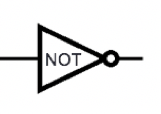
\includegraphics[height=0.5in]{../../resources/images/NOTx.png} \end{center}
\end{multicols}

%
 \vfill
\section*{Digital circuits basic examples}


{\bf Example digital circuit}: 

\begin{multicols}{2}
\begin{center}
   \includegraphics[width=1.2in]{../../resources/images/circuitEx.png} 
\end{center}
\columnbreak
Output when $x=1, y=0, z=0, w = 1$ is \underline{\phantom{$~~~0~~~$}}
Output when $x=1, y=1, z=1, w = 1$ is \underline{\phantom{$~~~0~~~$}}
Output when $x=0, y=0, z=0, w = 1$ is \underline{\phantom{$~~~0~~~$}}
\phantom{Output when $x=0, y=0, z=0, w = 0$ is \underline{\phantom{$~~~0~~~$}}}
\end{multicols}



Draw a logic circuit with inputs $x$ and $y$ whose output  is always $0$.  {\it  Can you use exactly 1 gate?}


\vspace{40pt} \vfill
\section*{Half adder circuit}


{\bf Fixed-width addition}: adding one bit at time, using the usual column-by-column and carry arithmetic, and dropping the carry from the leftmost column so the result is the same width as the summands.  In many cases, this gives representation of the correct value for the sum when we interpret the summands
in fixed-width binary or in 2s complement.

For single column:
\begin{center}
\begin{tabular}{cc|cc}
\multicolumn{2}{c|}{Input}  & \multicolumn{2}{|c}{Output}  \\
$x_0$ & $y_0$ & $c_0$ & $s_0$  \\
\hline
$1$ & $1$ & \phantom{$1$} & \phantom{$0$} \\
$1$ & $0$ & \phantom{$0$} & \phantom{$1$}\\
$0$ & $1$ & \phantom{$0$} & \phantom{$1$}\\
$0$ & $0$ & \phantom{$0$} & \phantom{$0$}\\
\end{tabular}
\end{center}

\begin{center}
\includegraphics[width=1.5in]{../../resources/images/half-adder.png}
\end{center} \vfill
\section*{Two bit adder circuit}


Draw a logic circuit that implements binary addition of 
two numbers that are each represented in fixed-width binary:
\begin{itemize}
\item Inputs  $x_0, y_0, x_1, y_1$ represent $(x_1  x_0)_{2,2}$ and $(y_1 y_0)_{2,2}$
\item Outputs  $z_0, z_1, z_2$ represent $(z_2  z_1 z_0)_{2,3} = (x_1  x_0)_{2,2} + (y_1 y_0)_{2,2}$ (may require up to width  $3$)
\end{itemize}

{\it First approach}: half-adder for each column, then combine carry from right column with sum of left column


Write expressions for the circuit output values in terms of input values:

$z_0 = \underline{\phantom{x_0 \oplus y_0\hspace{3in}}}$

$z_1 = \underline{\phantom{(x_1 \oplus y_1) \oplus c_0}\hspace{2.5in}}$ \phantom{where $c_0 = x_0 \land y_0$}

$z_2 = \underline{\phantom{(c_0 \land (x_1 \oplus y_1)) \oplus c_1}\hspace{2in}}$ \phantom{where $c_1 = x_1 \land y_1$}\\

\includegraphics[width=1.7in]{../../resources/images/width-2-adder.png}



{\it Second approach}: for middle column, first add carry from right column to $x_1$, then add result to $y_1$


Write expressions for the circuit output values in terms of input values:

$z_0 = \underline{\phantom{x_0 \oplus y_0}\hspace{3in}}$

$z_1 = \underline{ \phantom{(c_0 \oplus x_1) \oplus y_1}\hspace{2.4in}}$ \phantom{where $c_0 = x_0 \land y_0$}

$z_2 = \underline{\phantom{(c_0 \land x_1) \oplus ((c_0 \oplus x_1)\land y_1)}\hspace{1.5in}}$

\vfill

{\it Extra example} Describe how to generalize this addition circuit for larger width inputs.

 \vfill
\section*{Logical operators}


{\bf Logical operators} aka propositional connectives

\begin{tabular}{lccccp{4in}}
{\bf Conjunction} & AND & $\land$ &\verb|\land| & 2 inputs & Evaluates to $T$ exactly when {\bf both} inputs are $T$\\
{\bf Exclusive or} & XOR & $\oplus$ &\verb|\oplus| & 2 inputs & Evaluates to $T$ exactly when {\bf exactly one} of inputs is $T$\\
{\bf Disjunction} & OR & $\lor$ &\verb|\lor| & 2 inputs & Evaluates to $T$ exactly when {\bf at least one} of inputs is $T$\\
{\bf Negation} & NOT & $\lnot$ &\verb|\lnot| & 1 input & Evaluates to $T$ exactly when its input is $F$\\
\end{tabular} \vfill
\section*{Logical operators truth tables}


Truth tables: Input-output tables where we use $T$ for $1$ and $F$ for $0$.

\begin{center}
\begin{tabular}{cc||c|c|c}
\multicolumn{2}{c||}{Input}  & \multicolumn{3}{c}{Output} \\
& & {\bf Conjunction} &  {\bf Exclusive or} & {\bf Disjunction} \\
$p$ & $q$ & $p \land q$ &  $p  \oplus  q$ & $p \lor  q$ \\
\hline
$T$ & $T$ & $T$ & $F$ & $T$\\
$T$ & $F$ & $F$ & $T$ & $T$\\
$F$ & $T$ & $F$ & $T$ & $T$\\
$F$ & $F$ & $F$ & $F$ & $F$\\
\hline
& & \includegraphics[width=0.5in]{../../resources/images/xANDy.png}
&  \includegraphics[width=0.5in]{../../resources/images/xXORy.png}
&  \includegraphics[width=0.5in]{../../resources/images/xORy.png}
\end{tabular}
\qquad \qquad\qquad
\begin{tabular}{c||c}
Input & Output \\
& {\bf Negation} \\
$p$ & $\lnot p$ \\
\hline
$T$ & $F$ \\
$F$ & $T$\\
\hline & 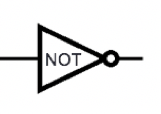
\includegraphics[width=0.5in]{../../resources/images/NOTx.png}
\end{tabular}
\end{center}
 \vfill
\section*{Logical operators example truth table}


\begin{center}
    \begin{tabular}{ccc||p{3in}|c|c}
    \multicolumn{3}{c||}{Input}  & \multicolumn{3}{c}{Output} \\
    $p$ & $q$ & $r$  &  &  $(p \land q) \oplus (~ ( p \oplus q) \land r~)$ & $(p \land q) \vee (~ ( p \oplus q) \land r~)$ \\
    \hline
    $T$ & $T$  & $T$ &   && \\
    $T$ & $T$  & $F$ &   && \\
    $T$ & $F$  & $T$ &   && \\
    $T$ & $F$  & $F$ &   && \\
    $F$ & $T$  & $T$ &   && \\
    $F$ & $T$  & $F$ &   && \\
    $F$ & $F$  & $T$ &   && \\
    $F$ & $F$  & $F$ &   && \\
    \end{tabular}
\end{center}
    \vfill \vfill
\section*{Truth table to compound proposition}


Given a truth table, how do we find an expression
using the input variables and logical operators that has the 
output values specified in this table?

{\it Application}: design a circuit given a desired input-output relationship.

\begin{center}
\begin{tabular}{cc||cc}
\multicolumn{2}{c||}{Input}  &\multicolumn{2}{c}{Output}\\
$p$ & $q$& $mystery_1$ & $mystery_2$\\
\hline
$T$ & $T$  & $T$ & $F$\\
$T$ & $F$  & $T$ & $F$\\
$F$ & $T$  & $F$ & $F$\\
$F$ & $F$  & $T$ & $T$\\
\end{tabular}
\end{center}


Expressions that have output $mystery_1$ are

\vspace{100pt}

Expressions that have output $mystery_2$ are

\vspace{100pt}
 \vfill
\section*{Dnf cnf definition}


{\bf  Definition} An expression built of variables and logical 
operators is in {\bf disjunctive normal form}  (DNF) means
that it is an OR of ANDs of variables and their negations.

{\bf  Definition} An expression built of variables and logical 
operators is in {\bf conjunctive normal form}  (CNF) means
that it is an AND of ORs of variables and their negations.
 \vfill
\section*{Dnf cnf example}




{\it Extra example}: An expression that has output ? is: 

\begin{tabular}{ccc||c}
    \multicolumn{3}{c||}{Input}  & Output\\
    $p$ & $q$ & $r$  &  ?\\
    \hline
    $T$ & $T$  & $T$ & $T$ \\
    $T$ & $T$  & $F$ & $T$ \\
    $T$ & $F$  & $T$ & $F$ \\
    $T$ & $F$  & $F$ & $T$ \\
    $F$ & $T$  & $T$ & $F$ \\
    $F$ & $T$  & $F$ & $F$ \\
    $F$ & $F$  & $T$ & $T$ \\
    $F$ & $F$  & $F$ & $F$ \\
\end{tabular}

\vfill

 \vfill
\section*{Compound proposition definitions}


{\bf Proposition}: Declarative sentence that is true or false (not both).

{\bf Propositional variable}: Variable that represents a proposition.

{\bf Compound proposition}: New proposition formed from existing propositions (potentially) using logical operators.
{\it Note}: A propositional variable is one example of a compound proposition.

{\bf Truth table}: Table with one row for each of the possible combinations of truth values of the input and 
    an additional column that shows the truth value of the result of the operation corresponding to a particular row.
    
 \vfill
\section*{Logical equivalence}


{\bf Logical equivalence }: Two compound  propositions are {\bf logically  equivalent} means that  they 
have the  same  truth  values for all settings of truth  values to their propositional  variables.

{\bf Tautology}:  A compound proposition that evaluates to true
for all settings of truth  values to its propositional  variables; it is  abbreviated $T$.

{\bf Contradiction}: A compound proposition that  evaluates  to  false 
for  all settings of truth  values to its propositional  variables; it  is abbreviated $F$.

{\bf Contingency}: A compound proposition that is neither a tautology nor a contradiction.
 \vfill
\section*{Tautology contradiction contingency examples}


Label each of the following as a tautology, contradiction, or contingency.

$p \land p$

$p \oplus p$

$p \lor p$

$p \lor \lnot p$

$p \land \lnot p$ \vfill
\section*{Logical equivalence extra example}


{\it Extra Example}: Which of the  compound propositions in the table below are logically equivalent?
\begin{center}
\begin{tabular}{cc||c|c|c|c|c}
\multicolumn{2}{c||}{Input}  & \multicolumn{5}{c}{Output} \\
$p$ & $q$ & $\lnot (p \land \lnot q)$ & $\lnot (\lnot p  \lor \lnot q)$ &  $(\lnot p \lor  q)$
& $(\lnot q \lor \lnot p)$ & $(p \land q)$  \\
\hline
$T$ & $T$ & &&&&\\
$T$ & $F$ & &&&&\\
$F$ & $T$ & &&&&\\
$F$ & $F$ & &&&&\\
\end{tabular}
\end{center} \vfill
\section*{Logical operators full truth table}


\begin{center}
    \begin{tabular}{cc||c|c|c|c|c}
    \multicolumn{2}{c||}{Input}  & \multicolumn{5}{c}{Output} \\
     & & Conjunction &  Exclusive or & Disjunction  &  Conditional & Biconditional  \\
    $p$ & $q$ & $p \wedge q$ &  $p  \oplus  q$ & $p \vee  q$ & $p \to q$ & $p \leftrightarrow q$\\
    \hline
    $T$ & $T$ & $T$ & $F$ & $T$ & $T$& $T$\\
    $T$ & $F$ & $F$ & $T$ & $T$ & $F$& $F$\\
    $F$ & $T$ & $F$ & $T$ & $T$ & $T$& $F$\\
    $F$ & $F$ & $F$ & $F$ & $F$ & $T$& $T$\\
    \hline
    && ``$p$ and $q$'' & ``$p$ xor $q$'' & ``$p$ or $q$'' & ``if $p$ then $q$'' & ``$p$ if and only if $q$''
    \end{tabular}
\end{center}
     \vfill
\section*{Hypothesis conclusion}


The only way to make  the conditional statement $p \to q$ false is to \underline{\phantom{\hspace{3in}}}\\

\begin{tabular}{llll}
The {\bf  hypothesis}  of $p \to q$ is  &\underline{\phantom{\hspace{1in}}} &
The {\bf  antecedent}  of $p \to q$ is  &\underline{\phantom{\hspace{1in}}} \\
&&&  \\
The {\bf  conclusion}  of $p \to q$ is & \underline{\phantom{\hspace{1in}}}&
The {\bf  consequent}  of $p \to q$ is & \underline{\phantom{\hspace{1in}}}\\
&&&  \\
\end{tabular}
 \vfill
\section*{Converse inverse contrapositive}


The {\bf converse}  of $p \to q$ is \underline{\phantom{ $q \to p$\hspace{1.6in}}}\\

The {\bf inverse}  of $p \to q$ is \underline{\phantom{ $\lnot p \to \lnot q$\hspace{1.6in}}}\\

The {\bf contrapositive}  of $p \to q$ is \underline{\phantom{$\lnot q \to \lnot p$\hspace{1.6in}}} \\
 \vfill
\section*{Compound propositions recursive definition}


We can use a recursive definition to describe all 
compound propositions that use propositional variables 
from a specified collection.  Here's the definition
for all compound propositions whose propositional variables 
are in $\{p, q\}$.

\[
\begin{array}{ll}
\textrm{Basis Step: } & p \textrm{ and } q \textrm{ are each a compound proposition} \\
\textrm{Recursive Step: } & \textrm{If } x \textrm{ is a compound proposition then so is } (\lnot x) 
\textrm{ and if } \\
& x \textrm{ and } y \textrm{ are both compound propositions then so is each of }\\
&(x \land y), (x \oplus y), (x \lor y), (x \to y), (x \leftrightarrow y)
\end{array}
\] \vfill
\section*{Compound propositions precedence}


Order of operations (Precedence) for logical operators: 

Negation, then conjunction / disjunction, then conditional / biconditionals.

Example: $\lnot p \lor \lnot q$ means $(\lnot p) \lor (\lnot q)$.
 \vfill
\section*{Logical equivalence identities}


{\bf (Some) logical equivalences}

{\it Can replace $p$ and $q$ with any compound proposition}

\begin{tabular}{llp{3in}}
$\lnot ( \lnot p) \equiv p$ & & {\bf Double negation}\\
&& \\
&& \\
$p \lor q \equiv q \lor p$ & $p \land q \equiv q \land p$ & {\bf Commutativity} Ordering of terms\\
&& \\
&& \\
$(p \lor q) \lor r  \equiv p \lor (q \lor r)$ & $(p \land q) \land r  \equiv p \land (q \land r)$ & {\bf Associativity} Grouping of terms\\
&& \\
&& \\
$p \land F \equiv F$ \qquad $p \lor T \equiv T$ & $p \land T \equiv p$ \qquad $p \lor F \equiv p$ & {\bf Domination} aka 
short circuit evaluation\\
&& \\
&& \\
$\lnot (p \land q) \equiv \lnot p \lor \lnot q$ & $\lnot (p \lor q) \equiv \lnot p \land\lnot q$  & {\bf DeMorgan's Laws}\\
&& \\
\end{tabular}

\begin{tabular}{llp{3in}}
$p \to q \equiv \lnot p \lor q$ & & \\
&& \\
&& \\
$p \to q \equiv \lnot q \to \lnot p$ & &{\bf Contrapositive} \\
&& \\
&& \\
$\lnot (p \to q) \equiv p\land \lnot q$  & &\\
&& \\
&& \\
$\lnot( p \leftrightarrow q) \equiv p \oplus q$ && \\
&& \\
&& \\
$p \leftrightarrow q \equiv q \leftrightarrow p$ &&\\
&& \\
\end{tabular}

{\it Extra examples}:

$p \leftrightarrow q$ is not logically equivalent to $p \land q$ because \underline{\phantom{\hspace{4in}}} 

$p \to q$ is not logically equivalent to $q \to p$ because \underline{\phantom{\hspace{4in}}} 
 \vfill
\section*{Logical operators english synonyms}


{\bf Common ways to express logical operators in English}:

{\bf Negation} $\lnot p$ can be said in English as 

\vspace{-20pt}
\begin{itemize}
\item Not $p$.
\item It's not the case that $p$.
\item $p$ is false.
\end{itemize}

{\bf Conjunction} $p \land q$ can be said in English as

\vspace{-20pt}
\begin{itemize}
    \item $p$ and $q$.
    \item Both $p$ and $q$ are true.
    \item $p$ but $q$.
\end{itemize}

{\bf Exclusive or} $p \oplus q$ can be said in English as

\vspace{-20pt}
\begin{itemize}
    \item $p$ or $q$, but not both.
    \item Exactly one of $p$ and $q$ is true.
\end{itemize}

{\bf Disjunction} $p \lor q$ can be said in English as

\vspace{-20pt}
\begin{itemize}
    \item $p$ or $q$, or both.
    \item $p$ or $q$ (inclusive).
    \item At least one of $p$ and $q$ is true.
\end{itemize}

{\bf Conditional} $p \to q$ can be said in English as

\begin{multicols}{2}
\begin{itemize}
    \item if $p$, then $q$.
    \item $p$ is sufficient for $q$.
    \item $q$ when $p$.
    \item $q$ whenever $p$.
    \item $p$ implies $q$.
    \item $q$ follows from $p$.
    \item $p$ is sufficient for $q$.
    \item $q$ is necessary for $p$.
    \item $p$ only if $q$.
\end{itemize}
\end{multicols}

{\bf Biconditional}

\vspace{-20pt}
\begin{itemize}
    \item $p$ if and only if $q$.
    \item $p$ iff $q$.
    \item If $p$ then $q$, and conversely.
    \item $p$ is necessary and sufficient for $q$.
\end{itemize} \vfill
\section*{Compound propositions translation}


{\bf Translation}: Express each of the following sentences as compound propositions, using
the given propositions.

\begin{multicols}{2}
``A sufficient condition for the warranty to be good is that you bought the computer less than a year ago"
\columnbreak
\begin{align*}
w &\text{ is  ``the warranty is good"} \\
b &\text{ is  ``you bought the computer less than a year ago"} \\
\end{align*}
\end{multicols}
\vfill

\begin{multicols}{2}
``Whenever the message was sent from an unknown system, it is scanned for viruses."
\columnbreak
\begin{align*}
s &\text{ is  ``The message is scanned for viruses"} \\
u &\text{ is  ``The message was sent from an unknown system"} \\
\end{align*}
\end{multicols}
\vfill

\begin{multicols}{2}
``I will complete my to-do list only if I put a reminder in my calendar"
\columnbreak
\begin{align*}
d &\text{ is  ``I will complete my to-do list"} \\
c &\text{ is  ``I put a reminder in my calendar"} \\
\end{align*}
\end{multicols}
\vfill \vfill
\section*{Consistency def}


{\bf Definition}: A collection of  compound  propositions
is called {\bf consistent} if  there
is  an assignment  of  truth values
to  the  propositional variables that makes
each of the compound propositions  true.
 \vfill
\section*{Consistency example}


{\bf Consistency}: 
\begin{quote}
Whenever the system software is being upgraded, users cannot access the file system. 
If users can access the file system, then they can save new files. 
If users cannot save new files, then the system software is not being upgraded.
\end{quote}

\begin{enumerate}
\item Translate to symbolic compound propositions
\vfill
\item Look for some truth assignment to the propositional variables for which all the compound propositions output $T$
\vfill
\end{enumerate} \vfill
\section*{Algorithm redundancy}


Real-life representations are often prone to corruption.  Biological codes, like RNA, 
may mutate naturally\footnote{Mutations of specific RNA codons have been linked to many disorders and cancers.}
and during measurement; cosmic radiation and other ambient noise 
can flip bits in computer storage\footnote{This RadioLab podcast episode
goes into more detail on bit flips: \url{https://www.wnycstudios.org/story/bit-flip}}. 
One way to recover from corrupted data is to introduce or exploit redundancy. 

Consider the following algorithm to introduce redundancy in a string of $0$s and $1$s.
\begin{algorithm}[caption={Create redundancy by repeating each bit three times}]
procedure $\textit{redun3}$($a_{k-1} \cdots a_0$: a nonempty bitstring)
for $i$ := $0$ to $k-1$
  $c_{3i}$ := $a_i$
  $c_{3i+1}$ := $a_i$
  $c_{3i+2}$ := $a_i$
return $c_{3k-1} \cdots c_0$
\end{algorithm}

\begin{algorithm}[caption={Decode sequence of bits using majority rule on consecutive three bit sequences}]
procedure $\textit{decode3}$($c_{3k-1} \cdots c_0$: a nonempty bitstring whose length is an integer multiple of $3$)
for $i$ := $0$ to $k-1$
  if exactly two or three of $c_{3i}, c_{3i+1}, c_{3i+2}$ are set to $1$
    $a_i$ := 1
  else 
    $a_i$ := 0
return $a_{k-1} \cdots a_0$
\end{algorithm}

Give a recursive definition of the set of outputs of the $redun3$ procedure, $Out$,

\phantom{{\bf Basis step}: $000 \in Out$ and $111 \in Out$\\ {\bf Recursive step}: If $x \in Out$ then $x000 \in Out$ and $x111 \in Out$ (where $x000$ and $x111$ are the results of string concatenation).}


Consider the message $m = 0001$ so that the sender calculates $redun3(m) = redun3(0001) = 000000000111$.

Introduce $\underline{\phantom{~~4~~}} $
errors into the message so that the signal received by the 
receiver is $\underline{\phantom{010100010101}}$
but the receiver is still able to decode the original message.


{\it Challenge: what is the biggest number of errors you can introduce?} 

Building a circuit for lines 3-6 in $decode$ procedure: given three input bits, we need to determine whether the
majority is a $0$ or a $1$.

\begin{center}
\begin{multicols}{2}\begin{tabular}{ccc|c}
$c_{3i}$ & $c_{3i+1}$ & $c_{3i+2}$ & $a_i$ \\
\hline
$1$ & $1$ & $1$ & $\phantom{1}$ \\
$1$ & $1$ & $0$ & $\phantom{1}$ \\
$1$ & $0$ & $1$ & $\phantom{1}$ \\
$1$ & $0$ & $0$ & $\phantom{0}$ \\
$0$ & $1$ & $1$ & $\phantom{1}$ \\
$0$ & $1$ & $0$ & $\phantom{0}$ \\
$0$ & $0$ & $1$ & $\phantom{0}$ \\
$0$ & $0$ & $0$ & $\phantom{0}$ \\\\
\end{tabular}
\columnbreak

Circuit 
\end{multicols}
\end{center} \vfill
\section*{Cartesian product definition}


{\bf Definition}: The {\bf Cartesian product} of the sets $A$ and $B$, 
$A \times B$, is the set of all ordered pairs $(a, b)$, where $a \in A$ and $b \in B$. 
That is: $A \times B = \{(a, b) \mid (a \in A) \land (b \in B)\}$.
The Cartesian product of the sets $A_1, A_2, \ldots ,A_n$, denoted by 
$A_1 \times A_2 \times \cdots \times A_n$, is the
set of ordered n-tuples $(a_1, a_2,...,a_n)$, where $a_i$ belongs to 
$A_i$ for $i = 1, 2,\ldots,n$. That is,
\[
    A_1 \times A_2 \times \cdots \times A_n = \{(a_1, a_2,\ldots,a_n) \mid a_i \in A_i \textrm{ for } i = 1, 2,\ldots,n\}
\] \vfill
\section*{Algorithm rna mutation insertion deletion}


Recall that $S$ is defined as the set of all RNA strands, nonempty strings made of the bases in 
$B = \{\A,\U,\G,\C\}$. 
We define the functions 
\[
  \textit{mutation}: S \times \mathbb{Z}^+ \times B \to S
\qquad \qquad
  \textit{insertion}: S \times \mathbb{Z}^+ \times B \to S
\]
\[
  \textit{deletion}: \{ s\in S \mid rnalen(s) > 1\} \times \mathbb{Z}^+ \to S
  \qquad \qquad \textrm{with rules}
\]

\begin{algorithm}
procedure $\textit{mutation}$($b_1\cdots b_n$: $\textrm{a RNA strand}$, $k$: $\textrm{a  positive integer}$, $b$: $\textrm{an  element of } B$)
for $i$ := $1$ to $n$
  if $i$ = $k$
    $c_i$ := $b$
  else
    $c_i$ := $b_i$
return $c_1\cdots c_n$ $\{ \textrm{The return value is a RNA strand made of the } c_i \textrm{ values}\}$
\end{algorithm}

\begin{algorithm}
procedure $\textit{insertion}$($b_1\cdots b_n$: $\textrm{a RNA strand}$, $k$: $\textrm{a  positive integer}$, $b$: $\textrm{an  element of } B$)
if $k > n$
  for $i$ := $1$ to $n$
    $c_i$ := $b_i$
  $c_{n+1}$ := $b$
else 
  for $i$ := $1$ to $k-1$
    $c_i$ := $b_i$
  $c_k$ := $b$
  for $i$ := $k+1$ to $n+1$
    $c_i$ := $b_{i-1}$
return $c_1\cdots c_{n+1}$ $\{ \textrm{The return value is a RNA strand made of the } c_i \textrm{ values}\}$
\end{algorithm}

\begin{algorithm}
procedure $\textit{deletion}$($b_1\cdots b_n$: $\textrm{a RNA strand with } n>1$, $k$: $\textrm{a  positive integer}$)
if $k > n$
  $m$ := $n$
  for $i$ := $1$ to $n$
    $c_i$ := $b_i$
else
  $m$ := $n-1$
  for $i$ := $1$ to $k-1$ 
    $c_i$ := $b_i$
  for $i$ := $k$ to $n-1$
    $c_i$ := $b_{i+1}$
return $c_1\cdots c_m$ $\{ \textrm{The return value is a RNA strand made of the } c_i \textrm{ values}\}$
\end{algorithm}
 \vfill
\section*{Rna mutation insertion deletion example}


Trace the pseudocode to find the output of $\textit{mutation}(~ (\A\U\C, 3, \G) ~)$

\vspace{50pt}

Fill in the blanks so that $\textit{insertion}(~(\A\U\C, \underline{\phantom{3}}, \underline{\phantom{\G}})~) = \A\U\C\G$

\vspace{50pt}

Fill in the blanks so that $\textit{deletion}(~(\underline{\phantom{\G\G}}, \underline{\phantom{1}})~) =  \G$

\vspace{50pt}
 \vfill
\section*{Predicate definition}


{\bf  Definition}: A  {\bf predicate}  is  a function from a given set (domain) to $\{T,F\}$.

A predicate can be applied, or {\bf evaluated} at, an element of the domain.

Usually, a predicate {\it describes a  property} that domain elements may or may not have.

Two predicates over the same domain are {\bf equivalent} means they evaluate to
the same truth values for all possible assignments of domain elements to the
input. In other words, they are equivalent means that they are equal as functions.

To define a predicate, we must specify its domain and its value at each domain element.
The rule assigning truth values to domain elements can be specified using a formula, 
English description, in a table (if the domain is finite), or recursively (if the domain is recursively
defined). \vfill
\section*{Predicate examples finite domain}


\begin{center}
    \begin{tabular}{c||c|c|c}
    Input & \multicolumn{3}{c}{Output} \\
    &$V(x)$ & $N(x)$ & $Mystery(x)$\\
    $x$ & $[x]_{2c,3} > 0$ & $[x]_{2c,3} < 0$& \\
    \hline
    $000$  & $F$ & & $T$\\
    $001$  & $T$ & & $T$\\
    $010$  & $T$ & & $T$\\
    $011$  & $T$ & & $F$\\
    $100$  & $F$ & & $F$\\
    $101$  & $F$ & & $T$\\
    $110$  & $F$ & & $F$\\
    $111$  & $F$ & & $T$\\
    \end{tabular}
    \end{center}
    
    The domain for each of the predicates $V(x)$, $N(x)$, $Mystery(x)$ is
    \underline{\phantom{$\{ b_1b_2b_3 ~\mid~ b_i \in \{0,1\} \textrm{ for each } i, 1 \leq i \leq 3 \}$}}.

    Fill in the table of values for the predicate $N(x)$ based on the formula given. \vfill
\section*{Predicate truth set definition}


{\bf Definition}: The {\bf truth  set} of a  predicate is the collection of all elements in its
domain where the predicate evaluates to $T$.

Notice that specifying the domain and the truth set is sufficient for defining
a predicate. \vfill
\section*{Predicate truth set example}


The truth set for the predicate $V(x)$ is $\underline{\phantom{\{ x ~\mid~ V(x) = T\} = \{ 001, 010, 011 \}}}$.

The truth set for the predicate $N(x)$ is $\underline{\phantom{\{ x ~\mid~ N(x) = T\} = \{ 101, 111 \}}}$.

The truth set for the predicate $Mystery(x)$ is $\underline{\phantom{\{ x ~\mid~ Mystery(x) = T\} = \{ 000, 001, 010, 101, 111 \}}}$.


\vfill \vfill
\section*{Quantification definition}


The {\bf universal quantification} of predicate $P(x)$ over
domain $U$ is the statement ``$P(x)$ for all values of $x$ in the domain $U$''
and is written $\forall x P(x)$ or $\forall x \in U ~P(x)$. 
When the domain is finite, universal quantification over the domain 
is equivalent to iterated {\it conjunction} (ands).

The {\bf existential quantification} of predicate $P(x)$ 
over domain $U$ is the statement ``There exists an element $x$ 
in the domain $U$ such that $P(x)$'' and is written $\exists x P(x)$
for $\exists x \in U ~P(x)$. 
When the domain is finite, existential quantification over the domain 
is equivalent to iterated {\it disjunction} (ors).

An element for which $P(x) = F$ is called a {\bf counterexample} of $\forall x P(x)$.

An element for which $P(x) = T$ is called a {\bf witness} of $\exists x P(x)$.
 \vfill
\section*{Quantification logical equivalence}


Statements involving predicates and quantifiers are {\bf logically equivalent} 
means they have the same truth value no matter which predicates (domains and functions) 
are substituted in. 

{\bf Quantifier version of De Morgan's laws}: 
$\boxed{\neg \forall x P(x) ~\equiv~ \exists x \left( \neg P(x) \right)}$
\qquad
\qquad
$\boxed{\neg \exists x Q(x) ~\equiv~ \forall x \left( \neg Q(x) \right)}$
 \vfill
\section*{Quantification examples finite domain}


Examples of quantifications using $V(x), N(x), Mystery(x)$:

{\bf True} or {\bf False}: $\exists x~ (~V(x) \land N(x)~)$

{\bf True} or {\bf False}: $\forall x~ (~V(x) \to N(x)~)$

{\bf True} or {\bf False}: $\exists x~ (~N(x) \leftrightarrow Mystery(x)~)$

Rewrite $\lnot \forall x~(~V(x) \oplus Mystery(x)~)$ into a logical equivalent statement.

\vspace{50pt}


Notice that these are examples where the predicates have {\it finite} domain.
How would we evaluate quantifications where the domain may be infinite? \vfill
\section*{Predicate rna example}


{\bf Example predicates on $S$, the set of RNA strands (an infinite set)}


$H: S \to \{T, F\}$ where $H(s) = T$ for all $s$.

Truth set of $H$ is \underline{\phantom{$S$\hspace{1in}}}\\

$F_{\A}: S \to \{T, F\}$  defined recursively by: 

~~Basis step: $F_{\A}(\A) = T$, $F_{\A}(\C) = F_{\A}(\G) = F_{\A}(\U) = F$

~~Recursive step: If $s \in S$ and $b \in B$, then $F_{\A}(sb) = F_{\A}(s)$.

Example where $F_{\A}$ evaluates to $T$ is \underline{\phantom{$\A\C\G$~\hspace{1in}}}

Example where $F_{\A}$ evaluates to $F$ is \underline{\phantom{$\U\A\C\U$\hspace{1in}}} \vfill
\section*{Rna rnalen basecount definitions}


{\it Recall the definitions}: The set of RNA strands $S$ is defined (recursively) by:
\[
\begin{array}{ll}
\textrm{Basis Step: } & \A \in S, \C \in S, \U \in S, \G \in S \\
\textrm{Recursive Step: } & \textrm{If } s \in S\textrm{ and }b \in B \textrm{, then }sb \in S
\end{array}
\]
where $sb$ is string concatenation.

The function \textit{rnalen} that computes the length of RNA strands in $S$ is defined recursively by:
\[
\begin{array}{llll}
& & \textit{rnalen} : S & \to \mathbb{Z}^+ \\
\textrm{Basis Step:} & \textrm{If } b \in B\textrm{ then } & \textit{rnalen}(b) & = 1 \\
\textrm{Recursive Step:} & \textrm{If } s \in S\textrm{ and }b \in B\textrm{, then  } & \textit{rnalen}(sb) & = 1 + \textit{rnalen}(s)
\end{array}
\]

The function \textit{basecount} that computes the number of a given base 
$b$ appearing in a RNA strand $s$ is defined recursively by:
\[
\begin{array}{llll}
& & \textit{basecount} : S \times B & \to \mathbb{N} \\
\textrm{Basis Step:} &  \textrm{If } b_1 \in B, b_2 \in B & \textit{basecount}(~(b_1, b_2)~) & =
        \begin{cases}
            1 & \textrm{when } b_1 = b_2 \\
            0 & \textrm{when } b_1 \neq b_2 \\
        \end{cases} \\
\textrm{Recursive Step:} & \textrm{If } s \in S, b_1 \in B, b_2 \in B &\textit{basecount}(~(s b_1, b_2)~) & =
        \begin{cases}
            1 + \textit{basecount}(~(s, b_2)~) & \textrm{when } b_1 = b_2 \\
            \textit{basecount}(~(s, b_2)~) & \textrm{when } b_1 \neq b_2 \\
        \end{cases}
\end{array}
\] \vfill
\section*{Predicates example rnalen basecount}


{\bf Using functions to define predicates}:

\fbox{\parbox{\textwidth}{
$L$ with domain $S \times \mathbb{Z}^+$ is defined by, for $s \in S$ and $n \in \mathbb{Z}^+$,
\[
L( ~(s, n)~) = \begin{cases}
T &\qquad\text{if $rnalen(s) = n$}\\
F &\qquad\text{otherwise}\\
\end{cases}
\]
In other words, $L(~(s,n)~)$ means $rnalen(s) = n$
}}

\fbox{\parbox{\textwidth}{
$BC$ with domain $S \times B \times \mathbb{N}$ is defined by, 
for $s \in S$ and $b \in B$ and $n \in \mathbb{N}$,
\[
BC(~(s, b, n)~) = \begin{cases}
T &\qquad\text{if $basecount(~(s,b)~) = n$}\\
F &\qquad\text{otherwise}\\
\end{cases}
\]
In other words, $BC(~(s,b,n)~)$ means $basecount(~(s,b)~) = n$
}}


Example where $L$ evaluates to $T$: $\underline{\phantom{(\A, 1)\hspace{1in}}}$  Why?

Example where $BC$ evaluates to $T$: $\underline{\phantom{(\A, \A1)\hspace{1in}}}$  Why?

Example where $L$ evaluates to $F$: $\underline{\phantom{(\A, 2)\hspace{1in}}}$ Why?

Example where $BC$ evaluates to $F$: $\underline{\phantom{(\A, \C, 1)\hspace{1in}}}$ Why? 

\fbox{\parbox{\textwidth}{
\[\exists t ~BC(t) \qquad \qquad 
\exists (s,b,n) \in S \times B \times \mathbb{N}~ (basecount(~(s,b)~) = n)\]

In English: \phantom{There exists an ordered $3$-tuple 
at which the predicate $BC$ evaluates to $T$.}

\vspace{30pt}

Witness that proves this existential quantification is true:\phantom{$(\G\G, \G, 2)$ or $(\G\A\U\G, \G, 2)$)}
}}

\fbox{\parbox{\textwidth}{
\[\forall t ~BC(t) \qquad \qquad 
\forall(s,b,n) \in S \times B \times \mathbb{N} ~(basecount(~(s,b)~) = n)\]

In English:\phantom{For all ordered $3$-tuples
the predicate $BC$ evaluates to $T$.}

\vspace{30pt}

Counterexample that proves this universal quantification is false: \phantom{$(\G\G, \A, 2)$ or $(\G\A\U\G, \G, 3)$)}
}}
 \vfill
\section*{Predicates projecting example rna basecount}


{\bf New predicates from old}
\begin{enumerate}
\item Define the {\bf new} predicate with domain $S \times B$ and rule
\[
basecount(~(s,b)~) = 3
\]
Example domain element where predicate is $T$: \phantom{$(\A\U\A\A, \A)$}\\

\item Define the {\bf new} predicate with domain $S \times \mathbb{N}$ and rule
\[
basecount(~(s,\A)~) = n
\]
Example domain element where predicate is $T$: \phantom{$(\A\U\A,2)$}\\

\item Define the {\bf new} predicate with domain $S \times B$ and rule
\[
\exists n \in \mathbb{N} ~(basecount(~(s,b)~) = n)
\]
Example domain element where predicate is $T$: \phantom{$(\A\U\A,\A)$}\\

\item Define the {\bf new} predicate with domain $S$ and rule
\[
\forall b \in B ~(basecount(~(s,b)~) = 1)
\]
Example domain element where predicate is $T$: \phantom{$\A\C\G\U$}\\
\end{enumerate} \vfill
\section*{Predicate notation}


{\bf Notation}: for a predicate $P$ with domain $X_1 \times \cdots \times X_n$ and a 
$n$-tuple $(x_1, \ldots, x_n)$ 
with each $x_i \in X$, we 
can write $P(x_1, \ldots, x_n)$ to mean $P( ~(x_1, \ldots, x_n)~)$.
 \vfill
\section*{Nested quantifiers}


{\bf Nested quantifiers}

\fbox{\parbox{\textwidth}{
\[
    \forall s \in S ~\forall b \in B ~\forall n \in \mathbb{N} ~(basecount(~(s,b)~) = n)
\]

In English: \phantom{There exists an ordered $3$-tuple 
at which the predicate $BC$ evaluates to $T$.}

\vspace{30pt}

Counterexample that proves this universal quantification is false:
\phantom{$(\G\G, \G, 3)$ or $(\G\A\U\G, \G, 2)$)}

\vspace{30pt}

}}

\fbox{\parbox{\textwidth}{
\[
    ~\forall n \in \mathbb{N} ~\forall s \in S ~\forall b \in B  ~(basecount(~(s,b)~) = n)
\]

In English: \phantom{There exists an ordered $3$-tuple 
at which the predicate $BC$ evaluates to $T$.}

\vspace{30pt}

Counterexample that proves this universal quantification is false:
\phantom{$(\G\G, \G, 3)$ or $(\G\A\U\G, \G, 2)$)}

\vspace{30pt}

}} \vfill
\section*{Alternating quantifiers strategies rna examples}


{\bf Alternating nested quantifiers}

\fbox{\parbox{\textwidth}{
$$\forall s \in S ~\exists b\in B ~(~basecount(~(s,b)~) = 3~)$$

In English: For each RNA strand there is a base that occurs 3 times in this strand.\\

Write the negation and use De Morgan's law to find a 
logically equivalent version where the negation is applied only to the 
$BC$ predicate (not next to a quantifier).

\vspace{60pt}


Is the original statement {\bf True} or {\bf False}?

}}

\fbox{\parbox{\textwidth}{

$$\exists s \in S ~\forall b \in B ~\exists n \in \mathbb{N} ~(~basecount(~(s,b)~) = n~)$$

In English: There is an RNA strand so that for each base there is some nonnegative
integer that counts the number of occurrences of that base in this strand.\\

Write the negation and use De Morgan's law to find a 
logically equivalent version where the negation is applied only to the 
$BC$ predicate (not next to a quantifier).

\vspace{60pt}


Is the original statement {\bf True} or {\bf False}?

}}
 \vfill
\section*{Proof strategies road map}


We now have propositional and predicate logic that can help us express 
statements about any domain. We will develop proof strategies to 
craft valid argument for proving that such statements are true or disproving
them (by showing they are false). We will practice these strategies with 
statements about sets and numbers, both because they are familiar and because they
can be used to build cryptographic systems. Then we will apply proof strategies
more broadly to prove statements about data structures and machine learning 
applications. \vfill
\section*{Proof strategies quantification finite domain}


When a predicate $P(x)$ is over a {\bf finite} domain:
\begin{itemize}
\item To show that $\forall x  P(x)$ is true: check that $P(x)$ evaluates to $T$ at each domain element by evaluating over and over.
\item To show that $\forall x  P(x)$ is false: find one counterexample, a domain element where $P(x)$ evaluates to $F$.
\item To show that $\exists x  P(x)$ is true: find one witness, a domain element where $P(x)$ evaluates to $T$.
\item To show that $\exists x  P(x)$ is false: check that $P(x)$ evaluates to $F$ at each domain element by evaluating over and over.
\end{itemize} \vfill
\section*{Proof strategy universal exhaustion}


\fbox{\parbox{\linewidth}{New! {\bf Proof of universal by exhaustion}: To prove that $\forall x \, P(x)$
is true when $P$ has a finite domain, evaluate the predicate at {\bf each} domain element to confirm that it is always T.
}} \vfill
\section*{Proof strategy universal generalization}


\fbox{\parbox{\linewidth}{

{\bf New! Proof by universal generalization}: To prove that $\forall x \, P(x)$
is true, we can take an arbitrary element $e$ from the domain of 
quantification and show that $P(e)$ is true, without making any assumptions about $e$ 
other than that it comes from the domain.


An {\bf arbitrary} element of a set or domain is a fixed but unknown element from that set. 
}}
 \vfill
\section*{Sets definitions}


{\bf Definitions}:

A {\bf set} is an  unordered collection of  elements.
When $A$ and  $B$ are sets,  $A = B$ (set equality) means  
\[
    \forall x  ( x\in A \leftrightarrow x \in B)
\]

When $A$ and  $B$ are sets, $A \subseteq B$ (``$A$ is a {\bf subset} of $B$") means 
\[
    \forall x  (x \in A  \to x  \in B)
\]

When $A$ and  $B$ are sets,  $A \subsetneq B$ (``$A$ is a {\bf proper subset} of $B$") means 
\[
    (A\subseteq B) \wedge  (A \neq B)
\] \vfill
\section*{Proof strategies conditionals}


\fbox{\parbox{\linewidth}{

{\bf New! Proof of conditional by direct proof}: To prove that the conditional statement $p \to q$ is true, 
we can assume $p$ is true and use that assumption to show $q$ is true.
}}

\fbox{\parbox{\linewidth}{

{\bf New! Proof of conditional by contrapositive proof}: To prove that the implication $p \to q$ is true, 
we can assume $q$ is false and use that assumption to show $p$ is also false.
}}

\fbox{\parbox{\linewidth}{

{\bf New! Proof of disjuction using equivalent conditional}: To prove that the 
disjunction $p \lor q$ is true, we can rewrite it equivalently as $\lnot p \to q$ and
then use direct proof or contrapositive proof.
}} \vfill
\section*{Proof strategies proof by cases}


\fbox{\parbox{\linewidth}{{\bf New! Proof by Cases}: To prove $q$, we can 
work by cases by first describing all possible cases we might be in
and then showing that each one guarantees $q$.
Formally, if we know that $p_1 \lor p_2$ is true, 
and we can show that $(p_1 \to q)$ is true and we can show that $(p_2 \to q)$, 
then we can conclude $q$ is true.
}} \vfill
\section*{Proof strategies ands}


\fbox{\parbox{\linewidth}{
{\bf New! Proof of conjunctions with subgoals}:
To show that $p \land q$ is true, we have two subgoals: subgoal (1) prove $p$ 
is  true; and, subgoal (2) prove $q$ is true.

\vspace{1em}

 To show that $p \land q$ is false, it's enough to prove that $\lnot p$.
 
 To show that $p \land q$ is false, it's enough to prove that $\lnot q$.
}} \vfill
\section*{Sets proof strategies}


To prove that one set is a subset of another, e.g. to show $A \subseteq B$:

\vspace{50pt}

To prove that two sets are equal, e.g. to show $A = B$:

\vspace{50pt}
 \vfill
\section*{Sets equality example}


Example: $\{ 43, 7, 9 \} = \{ 7, 43, 9, 7\}$

\vspace{50pt}
 \vfill
\section*{Sets basic proofs}


{\bf Prove} or {\bf  disprove}: $\{ \A,  \C,  \U,  \G\} \subseteq \{ \A\A, \A\C, \A\U, \A\G \}$ 

\vspace{150pt}

{\bf Prove} or {\bf  disprove}: For some set $B$, $\emptyset \in B$.

\vspace{150pt}

{\bf Prove} or {\bf  disprove}: For every set $B$, $\emptyset \in B$.

\vspace{150pt}

{\bf Prove} or {\bf  disprove}: The empty set is a subset of every set.

\vspace{150pt}

{\bf Prove} or {\bf  disprove}: The empty set is a proper subset of every set.

\vspace{150pt}

{\bf Prove} or {\bf  disprove}: $\{ 4, 6 \} \subseteq \{ n \mid  \exists c \in \mathbb{Z} ( n = 4c) \} $

\vspace{150pt}

{\bf Prove} or {\bf  disprove}: $\{ 4, 6 \} \subseteq \{ n ~\textbf{mod}~10 \mid  \exists c \in \mathbb{Z} ( n = 4c) \} $

\vspace{150pt}

 \vfill
\section*{Proofs signposting}


\fbox{\parbox{\textwidth}{

\vspace{10pt}

Consider \ldots, an {\bf arbitrary} \ldots.
{\bf Assume} \ldots, we {\bf want to show} that \ldots. Which is what was needed,
so the proof is complete $\square$.

\vspace{20pt} {\it or, in other words:} \vspace{20pt}

Let \ldots be an {\bf arbitrary} \ldots. {\bf Assume} \ldots, {\bf WTS} that \ldots {\bf QED}.

\vspace{10pt}

}} \vfill
\section*{Set operations union intersection powerset}


{\bf Cartesian product}: When $A$ and  $B$ are sets, 
\[
    A \times  B = \{ (a,b) \mid a \in A  \wedge b  \in B \}
\]

Example: $\{43, 9\} \times  \{9, \mathbb{Z}\}  = $
    
Example: $\mathbb{Z} \times \emptyset  = $

{\bf Union}: When $A$ and  $B$ are sets,
\[
    A \cup  B = \{ x \mid x \in A  \vee x \in B \}
\]    
    
Example: $\{43, 9\} \cup \{9, \mathbb{Z}\}  = $

Example: $\mathbb{Z} \cup \emptyset  = $ 

{\bf Intersection}: When $A$ and  $B$ are sets,
\[
    A \cap  B = \{ x \mid x \in A  \wedge x \in B \}
\]    
Example: $\{43, 9\} \cap \{9,\mathbb{Z}\}  = $

Example: $\mathbb{Z} \cap \emptyset  = $


{\bf Set  difference}: When $A$ and  $B$ are sets,

\[
    A -  B = \{ x \mid x \in A  \wedge x \notin B \}
\]

Example: $\{43, 9\} - \{9, \mathbb{Z}\}  = $

Example: $\mathbb{Z} - \emptyset  = $

    
{\bf Disjoint sets}: sets $A$ and  $B$ are disjoint means $A \cap  B  = \emptyset$

Example: $\{43, 9\}, \{9, \mathbb{Z}\}$ are not  disjoint 

Example: The sets $\mathbb{Z}$ and $\emptyset$ are disjoint

    

{\bf Power set}: When $U$ is a set, $\mathcal{P}(U) = \{ X \mid X \subseteq U\}$

Example: $\mathcal{P}(\{43, 9\}) = $

Example: $\mathcal{P}(\emptyset) = $
 \vfill
\section*{Sets basic proofs operations}


Let $W =  \mathcal{P}(  \{ 1,2,3,4,5\} )$


Example elements in $W$ are:
\vspace{20pt}

{\bf Prove} or {\bf  disprove}:  $\forall  A \in W\,  \forall B \in W\,  \left( A \subseteq B
~\to ~ \mathcal{P}(A) \subseteq \mathcal{P}(B) \right)$

\vfill
\vfill
\vfill

{\it Extra example}: {\bf Prove} or {\bf  disprove}:  $\forall  A \in W\,  \forall B \in W\,  \left( \mathcal{P}(A)  =\mathcal{P}(B)
~\to ~ A = B \right)$

\vspace{20pt}

{\it Extra example}: {\bf Prove} or {\bf  disprove}:  $\forall  A \in W\,  \forall B \in W\, \forall C  \in W\,  \left( A\cup B  = A \cup  C
~\to ~ B = C \right)$

\vspace{20pt} \vfill
\section*{Numbers facts}


\begin{enumerate}
    \item Addition and multiplication of real 
    numbers are each commutative and associative. 
    \vspace{25pt}
    \item The product of two positive numbers is positive, of 
    two negative numbers is positive, and of a positive and a negative number is negative.
    \vspace{25pt}
    \item The sum of two integers, the product of two integers, and the 
    difference between two integers are each integers.
    \vspace{25pt}
    \item For every integer $x$ there is no integer strictly between $x$ and $x+1$, 
    \vspace{25pt}
    \item When $x, y$ are positive integers, $xy \geq x$ and $xy \geq y$.
    \vspace{25pt}
\end{enumerate}
 \vfill
\section*{Factoring definition}


{\bf Definition}: When $a$ and $b$ are integers and $a$ is nonzero, 
{\bf $a$ divides $b$} means there is an integer $c$ such that $b = ac$ . 


Symbolically, $F(~(a,b)~) = \phantom{\exists c\in \mathbb{Z}~(b=ac)}$
and is  a predicate over the domain \underline{\phantom{$\mathbb{Z}^{\neq 0} \times \mathbb{Z}$}}


Other (synonymous) ways to say that $F(~(a,b)~)$ is true: 
\begin{center}
$a$ is a {\bf factor} of $b$
\qquad 
$a$ is a {\bf divisor} of $b$
\qquad  $b$ is a {\bf multiple} of $a$
\qquad
$a | b$
\end{center}

When $a$ is a positive integer and $b$ is any integer, $a | b$
exactly when $b \textbf{ mod } a = 0$

When $a$ is a positive integer and $b$ is any integer, $a | b$
exactly $b = a \cdot (b \textbf{ div } a)$ \vfill
\section*{Factoring translation examples}


{\it Translate these quantified statements by matching to English statement on right.}

\begin{multicols}{2}
$\exists a\in \mathbb{Z}^{\neq 0} ~(~F(~(a,a)~)~)$

$\exists a\in \mathbb{Z}^{\neq 0} ~(~\lnot F(~(a,a)~)~)$

$\forall a\in \mathbb{Z}^{\neq 0} ~(~F(~(a,a)~)~)$

$\forall a\in \mathbb{Z}^{\neq 0} ~(~\lnot F(~(a,a)~)~)$


Every nonzero integer is a factor of itself.

No nonzero integer is a factor of itself.

At least one nonzero integer is a factor of itself.

Some nonzero integer is not a factor of itself.
\end{multicols} \vfill
\section*{Factoring basic claims}


{\bf Claim}: Every nonzero integer is a factor of itself.

{\bf Proof}: 


\vspace{150pt}


{\bf Prove} or {\bf Disprove}: There is a nonzero integer that does not divide its square.



\vspace{150pt}

{\bf Prove} or {\bf Disprove}: Every positive factor of a positive integer is less than or equal to it.

\vspace{150pt}
 \vfill
\section*{Factoring basic claims continued}


{\bf Claim}: Every nonzero integer is a factor of itself and 
every nonzero integer divides its square.

\vspace{100pt}
 \vfill
\section*{Factoring even odd}


{\bf Definition}: an integer $n$ is {\bf even} means that there is an integer $a$ such that $n = 2a$; 
an integer $n$ is {\bf odd} means that there is an integer $a$ such that $n = 2a+1$.  Equivalently, 
an integer $n$ is {\bf even} means $n ~\textbf{ mod }~2 = 0$; an integer $n$ is {\bf odd} means $n ~\textbf{ mod }~2 = 1$.  
Also, an integer is even if and only if it is not odd.
 \vfill
\section*{Prime number definition}


{\bf Definition}:  An integer $p$ greater than $1$ is called {\bf prime} means 
the only positive factors of 
$p$ are $1$ and $p$. A positive integer that is greater than $1$ and is not prime 
is called composite. \vfill
\section*{Primes basic claims}


{\it Extra examples}: Use the definition to prove that $1$ is not prime, $2$ is prime, $3$
is prime, $4$ is not prime, $5$ is prime, $6$ is not prime, and $7$ is prime.


{\bf True or False}: The statement ``There are three consecutive positive integers that are prime."

{\it Hint}: These numbers would be of the form $p, p+1, p+2$ (where $p$ is a positive integer).

{\bf Proof}: We need to show \underline{\phantom{$\exists p \in \mathbb{Z}^+ ~(~Pr(p) \land Pr(p+1) \land Pr(p+2)~)$}}

\vspace{200pt}

{\bf True or False}: The statement ``There are three consecutive odd positive integers that are prime."

{\it Hint}: These numbers would be of the form $p, p+2, p+4$ (where $p$ is an odd positive integer).

{\bf Proof}: We need to show \underline{\phantom{$\exists p \in \mathbb{Z}^+ ~(~(p \textbf{ mod } 2 = 1 \land Pr(p) \land Pr(p+2) \land Pr(p+4)~)$}}

\vspace{200pt}
 \vfill
\section*{Rna rnalen basecount definitions}


{\it Recall the definitions}: The set of RNA strands $S$ is defined (recursively) by:
\[
\begin{array}{ll}
\textrm{Basis Step: } & \A \in S, \C \in S, \U \in S, \G \in S \\
\textrm{Recursive Step: } & \textrm{If } s \in S\textrm{ and }b \in B \textrm{, then }sb \in S
\end{array}
\]
where $sb$ is string concatenation.

The function \textit{rnalen} that computes the length of RNA strands in $S$ is defined recursively by:
\[
\begin{array}{llll}
& & \textit{rnalen} : S & \to \mathbb{Z}^+ \\
\textrm{Basis Step:} & \textrm{If } b \in B\textrm{ then } & \textit{rnalen}(b) & = 1 \\
\textrm{Recursive Step:} & \textrm{If } s \in S\textrm{ and }b \in B\textrm{, then  } & \textit{rnalen}(sb) & = 1 + \textit{rnalen}(s)
\end{array}
\]

The function \textit{basecount} that computes the number of a given base 
$b$ appearing in a RNA strand $s$ is defined recursively by:
\[
\begin{array}{llll}
& & \textit{basecount} : S \times B & \to \mathbb{N} \\
\textrm{Basis Step:} &  \textrm{If } b_1 \in B, b_2 \in B & \textit{basecount}(~(b_1, b_2)~) & =
        \begin{cases}
            1 & \textrm{when } b_1 = b_2 \\
            0 & \textrm{when } b_1 \neq b_2 \\
        \end{cases} \\
\textrm{Recursive Step:} & \textrm{If } s \in S, b_1 \in B, b_2 \in B &\textit{basecount}(~(s b_1, b_2)~) & =
        \begin{cases}
            1 + \textit{basecount}(~(s, b_2)~) & \textrm{when } b_1 = b_2 \\
            \textit{basecount}(~(s, b_2)~) & \textrm{when } b_1 \neq b_2 \\
        \end{cases}
\end{array}
\] \vfill
\section*{Alternating quantifiers proofs rna examples}


Which proof strategies could be used to prove each of the following statements?

{\it Hint: first translate the statements to English and identify the main logical structure.}

$\forall s \in S~(~rnalen(s) > 0~)$

\vspace{100pt}

$\forall b \in B~\exists s \in S~(~basecount(~(s,b)~)~ > 0~)$

\vspace{100pt}

$\forall s \in S ~\exists b\in B ~(~basecount(~(s,b)~) > 0~)$

\vspace{100pt}

$\exists s \in S \, (\textit{rnalen(s)} = \textit{basecount}(~(s, \A)~)$

\vspace{100pt}

$\forall s \in S \, (\textit{rnalen(s)} \geq \textit{basecount}(~(s, \A)~))$

\vspace{100pt}

 \vfill
\section*{Structural induction motivating example rna}


{\bf Claim} $\forall s \in S ~(~rnalen(s) > 0~)$

{\bf Proof}: Let $s$ be an arbitrary RNA strand. By the recursive definition of $S$,
either $s \in B$ or there is some strand $s_0$ and some base $b$ such that $s = s_0 b$.
We will show that the inequality holds for both cases.

{$\phantom{Basis}$} {\bf Case}: Assume $s \in B$. We need to show $rnalen(s) > 0$. 
By the basis step in the definition of $rnalen$,
$$rnalen(s) = 1$$
which is greater than $0$, as required.

{$\phantom{Recursive}$} {\bf Case}: Assume there is some strand $s_0$ and some base $b$ 
such that $s = s_0 b$. We will show {\it (the stronger claim)} that 
\[
    \forall u \in S ~\forall b \in B ~( ~\textit{rnalen}(u) >0  \to 
    \textit{rnalen}(ub) >0 ~)
\]
Consider an arbitrary RNA strand $u$ and an arbitrary base $b$, and assume towards a
direct proof,$~~{\phantom{ this is the induction hypothesis}}~~$ that
\[
    rnalen(u) > 0
\]
We need to show that $rnalen(ub) > 0$.
\[
    rnalen(ub) = 1 + rnalen (u) > 1 + 0 = 1 > 0
\]
as required. \vfill
\section*{Proof strategies structural induction}


\fbox{\parbox{\textwidth}{{\bf Proof by Structural Induction} 
To prove a universal quantification over a recursively defined set:
\begin{itemize}
    \item[] {\bf Basis Step}:  Show the statement holds for elements specified in the basis step of the definition.
    \item[]  {\bf Recursive Step}:  Show that if the statement is true for each of the elements used to construct
    new elements in the recursive step of the definition, the result holds for these new elements.
    \end{itemize}
}}
     \vfill
\section*{Structural induction example rnalen basecount}


{\bf Claim} $\forall s \in S \, (\textit{rnalen(s)} \geq \textit{basecount}(~(s, \A)~))$:

{\bf Proof}: We proceed by structural induction on the recursively defined set $S$.

{\bf Basis  Case}: We need to prove that 
the inequality holds for each element in the basis step of the recursive
definition of $S$. 
Need to show 
\begin{align*}
          &(~ rnalen(\A) \geq basecount(~(\A, \A)~)~) \land (~ rnalen(\C) \geq basecount(~(\C, \A)~)~) \\
    \land & (~ rnalen(\U) \geq basecount(~(\U, \A)~)~) \land (~ rnalen(\G) \geq basecount(~(\G, \A)~)~)
\end{align*}
We calculate, using the definitions of $rnalen$ and $basecount$:

\vspace{100pt}

{\bf Recursive Case}: We will prove that 
\[
    \forall u \in S ~\forall b \in B ~( ~rnalen(u) \geq basecount(~(u, \A)~) \to 
    rnalen(ub) \geq basecount(~(ub, \A)~)
\]

Consider arbitrary RNA strand $u$ and arbitrary base $b$. Assume, as the {\bf induction hypothesis},
that $rnalen(u) \geq basecount(~(u,\A)~)$. We need to show that $rnalen(ub) \geq basecount(~(ub, \A)~)$.

Using the recursive step in the definition of the function $rnalen$:
\[
    rnalen(ub) = 1 + rnalen(u)
\]
The recursive step in the definition of the function $basecount$ has two cases. We notice that 
$b = \A \lor b \neq \A$ and we proceed by cases.

{\it Case i.} Assume $b = \A$.

Using the first case in the recursive step in the definition of the function $basecount$:
\[
    basecount(~(ub, \A)~) = 1 + basecount(~(u,\A)~)
\]
By the {\bf induction hypothesis}, we know that $basecount(~(u,\A)~) \leq rnalen(u)$ so:
\[
    basecount(~(ub, \A)~) = 1 + basecount(~(u,\A)~) \leq 1 + rnalen(u) = rnalen (ub)
\]
and, thus, $basecount(~(ub,\A)~) \leq rnalen(ub)$, as required.

{\it Case ii.} Assume $b \neq \A$. 

Using the second case in the recursive step in the definition of the function $basecount$:
\[
    basecount(~(ub, \A)~) = basecount(~(u,\A)~)
\]
By the {\bf induction hypothesis}, we know that $basecount(~(u,\A)~) \leq rnalen(u)$ so:
\[
    basecount(~(ub, \A)~) = basecount(~(u,\A)~) \leq rnalen(u) < 1 + rnalen(u) = rnalen (ub)
\]
and, thus, $basecount(~(ub,\A)~) \leq rnalen(ub)$, as required.
 \vfill
\section*{Quiz basecount rnalen induction}


Recall the definitions of the functions $rnalen$ and $basecount$ from class.

\begin{enumerate}
    \item Select all and only options that give a witness for the existential quantification
    $$\exists s \in S ~(~rnalen(s) = basecount(~(s,\U)~)~)$$
    \begin{enumerate}
    \item $\A$
    \item $\U\U$
    \item $\C\U$
    \item $(\U, 1)$
    \item None of the above.
    \end{enumerate}
    
    \item Select all and only options that give a counterexample for the universal quantification
    $$\forall s \in S ~(~rnalen(s) > basecount(~(s,\G)~)~)$$
    \begin{enumerate}
    \item $\U$
    \item $\G\G$
    \item $\A\G$
    \item $\C\U\G$
    \item None of the above.
    \end{enumerate}
    
    \item Select all and only the true statements
    \begin{enumerate}
    \item $\forall s \in S ~\exists b \in B ~\left(~rnalen(s) = basecount(~(s,b)~)~ \right)$
    \item $\exists s \in S ~\forall b \in B ~\left(~rnalen(s) = basecount(~(s,b)~)~ \right)$
    \item \begin{align*} \forall s_1 \in S~\forall s_2 \in S ~&\forall b \in B ~\big( ~\big( rnalen(s_1) = basecount(~(s_1,b)~) \\
    &\land rnalen(s_2) = basecount(~(s_2,b)~) \land rnalen(s_1) = rnalen(s_2) \big) \to s_1 = s_2  \big)\end{align*}
    \item None of the above.
    \end{enumerate}
    
\end{enumerate} \vfill
\section*{Proofs signposting kinds of claims}


To organize our proofs, it's useful to highlight which claims are most important for 
our overall goals.
We use some terminology to describe different roles statements can have.

{\bf Theorem}: Statement that can be shown to be true, usually an important one.

Less important theorems can be called {\bf proposition}, {\bf fact}, {\bf result}, {\bf claim}.

{\bf Lemma}: A less important theorem that is useful in proving a theorem.
 
{\bf Corollary}: A theorem that can be proved directly after another one has been proved, 
without needing a lot of extra work.

{\bf Invariant}: A theorem that describes a property that is true about an algorithm or 
system no matter what inputs are used.




 \vfill
\section*{Structural induction example robot grid}


\begin{center}
    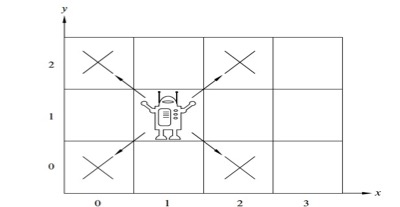
\includegraphics[width=3in]{../../resources/images/robot-grid.png}
\end{center}
    
{\bf Theorem}: A robot on an infinite 2-dimensional integer grid starts at $(0,0)$ and at each step moves
to diagonally adjacent grid point. This robot can / cannot {\footnotesize({\it circle one})} reach $(1,0)$.


{\bf Definition} The set of positions the robot can visit  $P$ is defined by:
\[
\begin{array}{ll}
    \textrm{Basis Step: } & (0,0) \in P \\
    \textrm{Recursive Step: } & \textrm{If } (x,y) \in P  \textrm{, then } 
    \phantom{(x+1, y+1), (x+1, y-1), (x-1, y-1), (x-1, y+1)} \textrm{ are also in } P
\end{array}
\]

{\it Example elements of $P$ are}:
\vspace{40pt}

{\bf Lemma}: $\forall (x,y) \in P( x+y \textrm{ is an even integer}~)$

{\it Why are we calling this a lemma?}


Proof of theorem using lemma: To show is $(1,0) \notin P$. Rewriting the lemma to explicitly 
restrict the domain of the universal, 
we have $\forall (x,y) ~(~ (x,y) \in P  \to (x+y \textrm{ is an even integer})~)$.  Since
the universal is true, 
$ (~ (1,0) \in P \to (1+0 \textrm{ is an even integer})~)$ is a true statement.
Evaluating the conclusion of this conditional statement: 
By definition of long division, since $1 = 0 \cdot 2 + 1$ (where $0 \in \mathbb{Z}$ and 
$1 \in \mathbb{Z}$ and $0 \leq 1 < 2$ mean that $0$ is the quotient and $1$ is the remainder), $1 ~\textrm{\bf mod}~ 2 = 1$ which is not $0$ 
so the conclusion is false.  A true conditional with a false conclusion must have a false hypothesis.
Thus, $(1,0) \notin P$, QED. $\square$

\vspace{20pt}

Proof of lemma by structural induction:

{\bf Basis Step}:

\vspace{100pt}


{\bf Recursive Step}:  Consider arbitrary $(x,y) \in P$.  To show is:
\[
(x+y \text{ is an even integer}) \to (\text{sum of coordinates of next position is even integer})
\]
Assume {\bf as the induction hypothesis, IH} that: 


\vspace{400pt} \vfill
\section*{Structural induction example sum of powers}


The set $\mathbb{N}$ is recursively defined.
Therefore, the function $sumPow: \mathbb{N} \to \mathbb{N}$
which computes, for input $i$, the sum of the nonnegative powers of $2$
up to and including exponent $i$ is defined
recursively by

\begin{alignat*}{2}
    \text{Basis step:  } \qquad & sumPow(0) = 1 &\\
    \text{Recursive step:  } & \text{If } x \in \mathbb{N} \text{, then } &sumPow(x+1) = sumPow(x) + 2^{x+1}
\end{alignat*}

$sumPow(0) =$

\vspace{20pt}

$sumPow(1) =$

\vspace{20pt}

$sumPow(2) =$

\vspace{20pt}


Fill in the blanks in the following proof of 
\[
    \forall n \in \mathbb{N}~(sumPow(n) = 2^{n+1} - 1)
\]

{\bf Proof}: Since $\mathbb{N}$ is recursively defined, we proceed by \underline{\phantom{structural induction \hspace{0.3in}}}.

{\bf Basis case}: We need to show that \underline{\phantom{$sumPow(0) = 2^{0+1} - 1$ \hspace{0.2in}}}.
Evaluating each side: $LHS = sumPow(0) = 1$ by the basis case in the recursive definition
of $sumPow$; $RHS = 2^{0+1} - 1 = 2^1 - 1 = 2-1 = 1$. Since $1=1$, the equality holds.

{\bf Recursive case}: Consider arbitrary natural number $n$ and assume, as the 
\underline{\phantom{Induction Hypothesis (IH)}} that $sumPow(n) = 2^{n+1} - 1$. We need to show that
\underline{\phantom{$sumPow(n+1) = 2^{(n+1) + 1} - 1$}}.  Evaluating each side: 
\[
LHS = sumPow(n+1) \overset{\text{rec def}}{=} sumPow(n)  + 2^{n+1}\overset{\text{IH}}{=} (2^{n+1} - 1) + 2^{n+1}.
\]
\[
RHS = 2^{(n+1)+1}- 1 \overset{\text{exponent rules}}{=} 2 \cdot 2^{n+1} -1  = \left(2^{n+1} + 2^{n+1} \right) - 1
\overset{\text{regrouping}}{=}  (2^{n+1} - 1) + 2^{n+1} 
\]
Thus, $LHS = RHS$. The structural induction is complete and we have proved the universal generalization.
$\square$

 \vfill
\section*{Proof strategy mathematical induction}


\fbox{\parbox{\textwidth}{

{\bf Proof by Mathematical Induction}

To prove a universal quantification over the set of all integers greater than
or  equal to some  base integer $b$,

\vspace{-10pt}

\begin{itemize}
\item[] {\bf Basis Step}:  Show the property holds for $b$. 
\item[]  {\bf Recursive Step}:  Consider an arbitrary integer $n$ greater than or  equal to  $b$, assume
    (as the {\bf induction hypothesis})  that the property holds  for $n$, and use  this and
    other facts to  prove that  the property holds for $n+1$.
\end{itemize}

}} \vfill
\section*{Linked lists definition}


{\bf Definition} The set of linked lists of natural numbers $L$ is defined recursively by
\[
\begin{array}{ll}
    \textrm{Basis Step: } & [] \in L \\
    \textrm{Recursive Step: } & \textrm{If } l \in L\textrm{ and }n \in \mathbb{N} \textrm{, then } (n, l) \in L
\end{array}
\] \vfill
\section*{Linked lists examples}


Visually:

\vspace{50pt}

Example: the list with two nodes whose first node has $20$ and whose second node
has $42$

\vspace{50pt} \vfill
\section*{Linked list length definition}


{\bf Definition}: The length of a linked list of natural numbers $L$, $length: L \to \mathbb{N}$ is defined by
\[
\begin{array}{llll}
\textrm{Basis Step:} &  & length(~[]~) &= 0 \\
\textrm{Recursive Step:} & \textrm{If } l \in L\textrm{ and }n \in \mathbb{N}\textrm{, then  } & length(~(n, l)~)  &= 1+ length(l)
\end{array}
\]
 \vfill
\section*{Linked lists prepend definition}


{\bf Definition}: The function $prepend : L \times \mathbb{N} \to L$ that adds an element at the 
front of a linked list is defined by
\[
\phantom{prepend(~(l, n)~) = (n, l)}
\]
 \vfill
\section*{Linked list append definition}


{\bf Definition} The function $append : L \times \mathbb{N} \to L$ that 
adds an element at the end of a linked list is defined by
\[
\begin{array}{llll}
\textrm{Basis Step:} & \textrm{If } m \in \mathbb{N}\textrm{ then } & \phantom{append(~([], m)~)} & \phantom{= (m, []) }\\
\textrm{Recursive Step:} & \textrm{If } l \in L\textrm{ and }n \in \mathbb{N}\textrm{ and }m \in \mathbb{N}\textrm{, then  } & \phantom{append(~(~(n, l), m~)~) } &\phantom{= (n, append(~(l, m)~)~)}
\end{array}
\] \vfill
\section*{Linked list append length claim proof}


{\bf Claim}: $\forall l \in L ~ (~length(~append(~(l, 100)~)~) > length(l)~)$

{\bf Proof:} By structural induction on $L$, we have two cases:

{\bf Basis Step}

    \begin{tabular}{l p{3.5in}}
     1. \textbf{To Show} $length(~append(~([], 100)~)~) > length(~[]~)$
    & Because $[]$ is the only element defined in the basis step of $L$, 
    we only need to prove that the property holds for $[]$.\\
    &  \\
     2. \textbf{To Show} $length(~(100,[])~) > length(~[]~)$
    &  By basis step in definition of $append$.\\
    &  \\
     3. \textbf{To Show} $(1 +length(~[]~)) > length(~[]~)$
    &  By recursive step in definition of $length$.\\
    &  \\    
     4. \textbf{To Show} $1+0 > 0$
    &  By basis step in definition of $length$.\\
    &  \\    
    5. $T$
    & By properties of integers \\
    &  \\    
    QED & Because we got to $T$ only by rewriting \textbf{To Show} to equivalent statements, using well-defined proof techniques, and applying definitions. \\
    \end{tabular}

{\bf Recursive Step}

Consider an arbitrary: $l' \in L$, $n \in \mathbb{N}$, and we  assume
as the {\bf induction hypothesis} that:
\[
length(~append(~(l', 100~)~)~) > length(l')
\]
Our goal is to show that $length(~append( ~(~(n,l'), 100~)~)~) > length(~(n,l')~)$ is also true. 
We start by working with
one side of the candidate inequality:
\begin{align*}
LHS &= length(~append( ~(~ (n,l'), 100~)~)~) \\
&= length(~(n, append(~(l', 100)~)~ )~) \qquad \text{by the recursive definition of $append$}\\
&= 1 + length(~ append(~(l', 100)~) ~) \qquad \text{by the recursive definition of $length$}\\
&> 1+ length(l')  \qquad \text{by the induction hypothesis}\\
&= length( (n,l') )  \qquad \text{by the recursive definition of $length$}\\
&= RHS 
\end{align*} \vfill
\section*{Linked list example each length}


Prove or disprove: $\forall n \in \mathbb{N} ~\exists l \in L ~(~length(l) = n~)$

\vspace{300pt} \vfill
\section*{Quiz linked list definitions}


Recall the definition of linked lists from class.

Consider this (incomplete) definition:

{\bf Definition} The function $\textit{increment} : \underline{\hspace{6em}}$ 
that adds 1 to the data in each node of a linked list is defined by:
\[
\begin{array}{llll}
& & \textit{increment} : \underline{\hspace{3em}} & \to \underline{\hspace{3em}} \\
\textrm{Basis Step:} & & \textit{increment}([]) & = [] \\
\textrm{Recursive Step:} & \textrm{If } l \in L, n \in \mathbb{N} & \textit{increment}((n, l)) & = (1 + n, \textit{increment}(l))
\end{array}
\]

Consider this (incomplete) definition:

{\bf Definition} The function $\textit{sum} : L \to \mathbb{N}$ that adds 
together all the data in nodes of the list is defined by:
\[
\begin{array}{llll}
& & \textit{sum} : L & \to \mathbb{N} \\
\textrm{Basis Step:} & & \textit{sum}([]) & = 0 \\
\textrm{Recursive Step:} & \textrm{If } l \in L, n \in \mathbb{N} & \textit{sum}((n, l)) & = \underline{\hspace{8em}}
\end{array}
\]

You will compute a sample function application and then fill in the 
blanks for the domain and codomain of each of these functions.

\begin{enumerate}
    \item Based on the definition, what is the result of $\textit{increment}((4, (2, (7, []))))$? Write your answer directly with no spaces.
    
    \item Which of the following describes the domain and codomain of \textit{increment}?
    
    \begin{multicols}{2}
    \begin{enumerate}
        \item The domain is $L$ and the codomain is $\mathbb{N}$
        \item The domain is $L$ and the codomain is $\mathbb{N} \times L$
        \item The domain is $L \times \mathbb{N}$ and the codomain is $L$
        \item The domain is $L \times \mathbb{N}$ and the codomain is $\mathbb{N}$
        \item The domain is $L$ and the codomain is $L$
        \item None of the above
    \end{enumerate}
    \end{multicols}
    
    \item Assuming we would like $sum((5, (6, [])))$ to evaluate to $11$ and $sum((3, (1, (8, []))))$ to evaluate to $12$, which of the following could be used to fill in the definition of the recursive case of \textit{sum}?
    
     \begin{multicols}{2}
    \begin{enumerate}
        \item $\begin{cases}
            1 + \textit{sum}(l) & \textrm{when } n \neq 0 \\
            \textit{sum}(l) & \textrm{when } n = 0 \\
        \end{cases}$
        \item $1 + \textit{sum}(l)$
        \item $n + \textit{increment}(l)$
        \item $n + \textit{sum}(l)$
        \item None of the above
    \end{enumerate}
    \end{multicols}
    
    \newpage
    \item Choose only and all of the following statements that are \textbf{well-defined}; that is, they correctly reflect the domains and codomains of the functions and quantifiers, and respect the notational conventions we use in this class. Note that a well-defined statement may be true or false.

    \begin{multicols}{2}    
    \begin{enumerate}
        \item $\forall l \in L \, (\textit{sum}(l))$
        \item $\exists l \in L \, (\textit{sum}(l) \land \textit{length}(l))$
        \item $\forall l \in L \, (\textit{sum}(\textit{increment}(l)) = 10)$
        \item $\exists l \in L \, (\textit{sum}(\textit{increment}(l)) = 10)$
        \item $\forall l \in L \, \forall n \in \mathbb{N} \, ((n \times l) \subseteq L)$
        \item $\forall l_1 \in L \, \exists l_2 \in L \, (\textit{increment}(\textit{sum}(l_1)) = l_2)$
        \item $\forall l \in L \, (\textit{length}(\textit{increment}(l)) = \textit{length}(l))$
    \end{enumerate}
    \end{multicols}
    
    \item Choose only and all of the statements in the previous part that are both well-defined and true.
\end{enumerate} \vfill
\end{document}